%% Use the standard UP-methodology class
%% with French language.
%%
%% You may specify the option 'twoside' or 'oneside' for
%% the document.
%%
%% See the documentation tex-upmethodology on
%% http://www.arakhne.org/tex-upmethodology/
%% for details about the macros that are provided by the class and
%% to obtain the list of the packages that are already included. 
 
\documentclass[english]{spimubphdthesis}
%\documentclass{report}
 
%%--------------------
%% The TeX code is entering with UTF8
%% character encoding (Linux and MacOS standards)
\usepackage[utf8]{inputenc}
 
%%-------------------
%% You want to use the NatBib extension
%\usepackage[authoryear]{natbib}
 
%%--------------------
%% Include the 'multibib' package to enable to
%% have different types of bibliographies in the
%% document (see at the end of this template for
%% an example with a personnal bibliography and
%% a general bibliography)
%%
%% Each bibliography defined with 'multibib'
%% adds a chapter with the corresponding
%% publications (in addition to the chapter for
%% the standard/general bibliography).
%% CAUTION:
%% There is no standard way to do include this type of
%% personnal bibliography.
%% We propose to use 'multibib' package to help you,
%% for example.
%\usepackage{multibib}
 
%% Define a "type" of bibliography, here the PERSONAL one,
%% that is supported by 'multibib'.
%\newcites{PERSO}{Liste de mes publications}
 
%% To cite one of your PERSONAL papers with the style
%% of the PERSONAL bibliography: \citePERSO{key}
%% To force to show one of your PERSONAL papers into
%% the PERSONAL bibliography, even if not cited in the
%% text: \nocitePERSO{key}
 
%% REMARK: When you are using 'multibib', you
%% must compile the PERSONAL bibliography by hand.
%% For example, the sequence of commands to run
%% when you had defined the bibliography PERSO is:
%%   $ pdflatex my_document.tex
%%   $ bibtex my_document.aux
%%   $ bibtex PERSO.aux
%%   $ pdflatex my_document.tex
%%   $ pdflatex my_document.tex
%%   $ pdflatex my_document.tex


%%--------------------
%% Add here any other packages that are needed for your document.
%\usepackage{eurosim}
%\usepackage{amsmath}
\usepackage{graphicx}
\usepackage{epsfig}
\usepackage{mathrsfs}
\usepackage{times}
\usepackage{makeidx}
\usepackage{amsmath}
\usepackage{algorithm}
\usepackage{algorithmic}
%\usepackage{subfigure}
%\usepackage{subcaption}
\usepackage{multicol}
\usepackage{array}
\usepackage{siunitx}
\usepackage{balance} % This allows for the even columns in the final page, just insert \balance in the last page, e.g., before the reference list
\usepackage{cite}
%\usepackage{setspace}
\usepackage{etoolbox}
\newtoggle{blindcopy}
%\toggletrue{blindcopy}
\usepackage{hhline}
\usepackage{booktabs}
\usepackage{rotating}
\usepackage{multirow}
\usepackage{wasysym}
\usepackage[subrefformat=parens,labelformat=parens]{subcaption}
\usepackage{xcolor}
\usepackage{adjustbox}

\usepackage{listings}
\lstset{
	basicstyle=\ttfamily,
	columns=fullflexible,
	breaklines=true,
	postbreak=\mbox{\textcolor{black}{$\hookrightarrow$}\space},
}

% set new command for table column width
\usepackage{array}
\newcolumntype{L}[1]{>{\raggedright\let\newline\\\arraybackslash\hspace{0pt}}m{#1}} % left aligned
\newcolumntype{C}[1]{>{\centering\let\newline\\\arraybackslash\hspace{0pt}}m{#1}} % center aligned
\newcolumntype{R}[1]{>{\raggedleft\let\newline\\\arraybackslash\hspace{0pt}}m{#1}} % right aligned

\usepackage{etoolbox}
\newtoggle{usingspim}
\toggletrue{usingspim}
%\togglefalse{usingspim}

\iftoggle{usingspim}
{
	% nothing
}
{
	%paragraph indentation
	\setlength{\parindent}{4em} 
	
	%paragraph spacing
	\setlength{\parskip}{1em}
	
	%Line spacing
	\renewcommand{\baselinestretch}{1.6}
}
 
%%--------------------
%% Set the title, subtitle, defense date, and
%% the registration number of the PhD thesis.
%% The optional parameter is the subtitle of the PhD thesis.
%% The first mandatory parameter is the title of the PhD thesis.
%% The second mandatory parameter is the date of the PhD defense.
%% The third mandatory parameter is the location/city of the PhD defense.
%% The forth mandatory parameter is the reference number given by
%% the University Library after the PhD defense.
\iftoggle{usingspim}{
\declarethesis[This is the sub-title]{Performance Estimation, Testing, and Control of Cyber-Physical Systems Employing Non-Ideal Communications Networks}{9 July 2020}{Dijon}{XXX}
}

 
%%--------------------
%% Set the author of the PhD thesis
\iftoggle{usingspim}{
\addauthor[rick.candell@gmail.com]{Richard}{Candell}
}

 
%%--------------------
%% Add a member of the jury
%%
%% CAUTION 1: If a Jury member is not present during the defense,
%%            she/he must be in the list of the Jury members.
%%            Only the reviewers and the members who are present during the defense must
%%            appear in the Jyry member list. 
%% CAUTION 2: After your defense, you must assign the role "Pr\'esident" to
%%            the Jury member who have been the President of the Jury.
%% CAUTION 3: The recommended order for the Jury members is:
%%            President, Reviewer(s), Examiner(s), Director(s),
%%            Other supervisor(s), Invited person(s).
%% \addjury{Firstname}{Lastname}{Role in the jury}{Position}
\iftoggle{usingspim}{
\addjury{Incroyable}{Hulk}{Pr\'esident}{Professeur à l'Université de Gotham City \\ Commentaire secondaire}
\addjury{Captain}{America}{Rapporteur}{Professeur à l'Université USA}
\addjury{Super}{Man}{Examinateur}{Professeur à l'Université de Gotham City}
\addjury{Bat}{Man}{Directeur de thèse}{Professeur à l'Université de Gotham City}
\addjury{The}{Volwerine}{Codirecteur de thèse}{Professeur à l'Université de Gotham City}
\addjury{Pac}{Man}{Invité}{Professeur quelque part}
}

 
%%--------------------
%% Change style of the table of the jury
%% \Set{jurystyle}{put macros for the style}
%\Set{jurystyle}{\small}
 
%%--------------------
%% Set the English abstract
\iftoggle{usingspim}{
\thesisabstract[english]{Lorem ipsum dolor sit amet, saepe quodsi dolores an usu. An sed fugit dissentiunt, ex tota soleat duo. Omnes deserunt adversarium qui ad, periculis pertinacia has id. Ea tibique antiopam eos. Usu illud cetero voluptatum ne, ea odio soluta labores sit.	Pri modus eruditi definiebas an. Dicat latine inermis no quo, eos tollit delicata interesset cu. Placerat vituperatoribus pro ne, cu verear tritani deterruisset usu. Quaeque recusabo maluisset te pri, mutat maiorum accusamus at his.	Pro ad nihil deleniti senserit, mundi feugiat indoctum an sea. In consulatu efficiendi qui, eu duo dicta deserunt definitiones, te atqui sapientem adolescens sit. Id pro consulatu splendide evertitur, vis eu perpetua molestiae, an melius virtute efficiantur vis. Animal aeterno mei ei.	Lucilius suavitate euripidis vis id, cu dicam ridens forensibus vis. In incorrupte adversarium pri, ut velit singulis nec, nisl facer dissentias ex duo. Id est nulla periculis, epicuri percipit cu eum. Praesent temporibus mediocritatem ex cum, his quot nonumy iriure ut, qui natum aliquip id. Interesset quaerendum repudiandae cum ea. Mazim perpetua deterruisset ne mei, cum esse novum minimum ea.}
}

 
%%--------------------
%% Set the English keywords. They only appear if
%% there is an English abstract
\iftoggle{usingspim}{
\thesiskeywords[english]{industrial wireless, factory communications, networked control, manufacturing}
}

 
%%--------------------
%% Set the French abstract
\iftoggle{usingspim}{
%\thesisabstract[french]{Lorem ipsum dolor sit amet, saepe quodsi dolores an usu. An sed fugit dissentiunt, ex tota soleat duo. Omnes deserunt adversarium qui ad, periculis pertinacia has id. Ea tibique antiopam eos. Usu illud cetero voluptatum ne, ea odio soluta labores sit.	Pri modus eruditi definiebas an. Dicat latine inermis no quo, eos tollit delicata interesset cu. Placerat vituperatoribus pro ne, cu verear tritani deterruisset usu. Quaeque recusabo maluisset te pri, mutat maiorum accusamus at his.	Pro ad nihil deleniti senserit, mundi feugiat indoctum an sea. In consulatu efficiendi qui, eu duo dicta deserunt definitiones, te atqui sapientem adolescens sit. Id pro consulatu splendide evertitur, vis eu perpetua molestiae, an melius virtute efficiantur vis. Animal aeterno mei ei.	Lucilius suavitate euripidis vis id, cu dicam ridens forensibus vis. In incorrupte adversarium pri, ut velit singulis nec, nisl facer dissentias ex duo. Id est nulla periculis, epicuri percipit cu eum. Praesent temporibus mediocritatem ex cum, his quot nonumy iriure ut, qui natum aliquip id. Interesset quaerendum repudiandae cum ea. Mazim perpetua deterruisset ne mei, cum esse novum minimum ea.}
}

 
%%--------------------
%% Set the French keywords. They only appear if
%% there is an French abstract
\iftoggle{usingspim}{
%\thesiskeywords[french]{Mot-cl\'e 1, Mot-cl\'e 2}
}

 
%%--------------------
%% Change the layout and the style of the text of the "primary" abstract.
%% If your document is written in French, the primary abstract is in French,
%% otherwise it is in English.
%\Set{primaryabstractstyle}{\tiny}
 
%%--------------------
%% Change the layout and the style of the text of the "secondary" abstract.
%% If your document is written in French, the secondary abstract is in English,
%% otherwise it is in French.
%\Set{secondaryabstractstyle}{\tiny}
 
%%--------------------
%% Change the layout and the style of the text of the "primary" keywords.
%% If your document is written in French, the primary keywords are in French,
%% otherwise they are in English.
%\Set{primarykeywordstyle}{\tiny}
 
%%--------------------
%% Change the layout and the style of the text of the "secondary" keywords.
%% If your document is written in French, the secondary keywords are in English,
%% otherwise they are in French.
%\Set{secondarykeywordstyle}{\tiny}
 
%%--------------------
%% Change the speciality of the PhD thesis
\iftoggle{usingspim}{
\Set{speciality}{Informatique}
}
 
%%--------------------
%% Change the institution
\iftoggle{usingspim}{
\Set{universityname}{Universit\'e de Bourgogne}
}
 

%%--------------------
%% Clear the list of the laboratories
\iftoggle{usingspim}{
\resetlaboratories
}

%%--------------------
%% Add the laboratory where the thesis was made
%\addlaboratory{Laboratoire Waynes Industry}
\iftoggle{usingspim}{
\addlaboratory{Laboratoire \'Electronique, Informatique et Image}
}


%%--------------------
%% Clear the list of the partner/sponsor logos
%\resetpartners

%%--------------------
%% Add the logos of the partners or the sponsors on the front page
%%
%% CAUTION 1: At least, the logo of the University should appear (UB)
%%
%\addpartner[image options]{image name}

%\addpartner{ub}

%%--------------------
%% Change the header and the foot of the pages.
%% You must include the package "fancyhdr" to
%% have access to these macros.
%% Left header
%\lhead{}
%% Center header
%\chead{}
%% Right header
%\rhead{}
%% Left footer
%\lfoot{}
%% Center footer
%\cfoot{}
%% Right footer
%\rfoot{}
 
%%--------------------
% Declare several theorems
\iftoggle{usingspim}{
\declareupmtheorem{mytheorem}{My Theorem}{List of my Theorems}
}
{
}

%%--------------------
%% Change the message on the backcover.
%\Set{backcovermessage}{%
%	Some text
%}

\begin{document}
 
%%--------------------
%% The following line does nothing until
%% the class option 'nofrontmatter' is given.
%\frontmatter

%%--------------------
%% The following line permits to add a chapter for "acknowledgements"
%% at the beginning of the document. This chapter has not a chapter
%% number (using the "star-ed" version of \chapter) to prevent it to
%% be in the table of contents
\chapter*{Acknowledgments}
The author would like express his gratitude to his beautiful daughter, Erin, for all of her generous support, kindness, and care, and her countless hours as a child hooking up wires and doing inventory of computer peripherals in my laboratory.  I hope that she remembers fondly those weekends listening to her Avengers movies while running factory simulators and troubleshooting robots.

Other acknowledgments: Mohammed, Yongkang, Karl




 
%%--------------------
%% Include a general table of contents
\iftoggle{usingspim}{
\tableofcontents


%%--------------------
%% The content of the PhD thesis
\mainmatter
}
 
\part{Context and Problem Statement}

\include{chapter-intro/chapter-intro}

\part{Technical Contributions}

\include{chapter-guidelines/chapter-guide}


\newcommand{\argmax}{\operatornamewithlimits{arg\ max}}
\newtheorem{theorem}{Theorem}[section]
\newtheorem{lemma}[theorem]{Lemma}
\newtheorem{property}[theorem]{Property}

\chapter{Industrial Wireless Technology And Applications}\label{chapter:reswk}

% Some very useful LaTeX packages include:
% (uncomment the ones you want to load)
	
\chapterintro*

The use of wireless technologies within factories demands a comprehensive understanding of the problems and potential solutions associated with the rigors of the manufacturing environment. A clearly defined problem space would significantly ease the selection and deployment of appropriate wireless solutions to connected factory systems.  A mapping of potential technologies to classes of use cases within the problem space will be useful to factory operators, system integrators, and wireless systems manufacturers.  Identification of use cases, not addressed by existing technologies, may be used to spur targeted innovation where reliability, resilience, latency, and scalability are joint concerns. Motivated by the industry need for independent practical guidelines and solutions to difficult wireless control problems, this chapter provides a classification of the problem categories where networking technologies may be deployed. It then maps specific technologies that may serve as interim or terminal solutions for those use cases identified within the problem space taxonomy. This chapter is intended to provide a detailed exposition of the requirements directed towards industrial wireless.  It draws on various sources of requirements captured by academic literature, industry organizations, and standards institutes.  The work therefore presents a picture of the requirements landscape at the beginning of this research.  Further work in this area can be found in~\cite{Montgomery2019} and~\cite{Raptis2019}.

	\section{Introduction} \label{sec:intro}
%    \subsection{Purpose}
    Industrial wireless is a key enabling technology for the Industrial Internet of Things (IIoT).  The IIoT promises lower costs of deployment, increased mobility of factory assets, massive interconnectivity, improved situational awareness, increased efficiency of the operation, and improved operations analytics.  IIoT and advanced manufacturing technology seek to improve competitiveness, productivity, and responsiveness to customer needs. However, it is often stated that where wireless is deployed, factory enhancements fail to meet expectations typically in areas of reliability, resilience, and scalability. Moreover, transmission security is often cited as an area of concern. Risk averse organizations will establish policies that preclude wireless to be deployed for specific types of applications such as feedback control or safety. Yet, factory operators are increasingly demanding that wireless be deployed for critical and sometimes perceivably dangerous applications.  For this reason, the
\iftoggle{blindcopy}{(BLIND COPY - NAME REMOVED)}{National Institute of Standards and Technology (NIST)} 
is developing best practice guidelines to help factory operators select appropriate wireless systems for their particular use case and then deploy that solution effectively.  Such a mission requires participation by factory operators, system integrators, and device manufacturers. A comprehensive taxonomy of the existing problem space within industry and a survey of existing and missing technologies are necessary to the success of such a mission. This chapter provides the author's classification of industrial wireless cases and links current technologies to those use cases if applicable. 
    
%    \subsection{Related Work}
%    %Mohamed will provide.  High level mentions and limitation.  Stop.
%The use of industrial wireless networks has been studied in many works in the literature. However, no comprehensive survey of the whole problem space of industrial communications has been performed.
%
%In \cite{6248648}, the authors have introduced a comparison between the commercial and industrial communications networks where an industrial network has been divided to five different levels. These levels include field equipment, controller level, application, supervisory, and external networks. The differences in requirements between different levels are discussed. Moreover, three types of information are considered which are control, diagnostic, and safety information as described in \cite{4118467}. However all these levels of industrial networks are mentioned in \cite{6248648}, the article focuses only on the manufacturing and instrumentation communications and does not consider other types of communications networks that exist in industrial environments. Also, in \cite{What}, three levels of communications are considered which are device, control, and information levels. Moreover, the current wired industrial technologies for these levels are discussed briefly.
%
%More works focused on the communications at the field devices level where sensing and control information is transfered. In \cite{7005074},  the communication between field devices has been studied where the requirements for a large number of nodes may not be achieved. The use of fieldbus solutions limit the scalability and resilience and hence industrial Ethernet capabilities are introduced in this article. Moreover, in \cite{Connectivity}, the communication for monitoring and control operations is discussed. A comparison between fieldbus technologies, industrial Ethernet, and wireless solutions is performed. The author has discussed the use of Wi-Fi, Bluetooth, ZigBee, and WirelessHART technologies in industrial applications. Similarly, the authors of \cite{6490786} considered the industrial communications networks requirements in process automation specifically at field devices level. Finally, in \cite{GE_Professional}, many case-studies are discussed for communication networks in industrial scenarios. Moreover, the design steps for these solutions are briefly discussed.

%    \subsection{Paper Organization}
%    The rest of the paper is organized as follows. The problem space for employing wireless networks is presented in Section II. Then, the technical considerations while designing industrial wireless networks are discussed briefly in Section III.  In Section IV, a mapping between the problem space and the current technology space is provided. Finally in Section V, future directions and conclusions are presented.
    
    \section{Problem Space}
    
    \subsection{Introduction and Success Considerations}
    Implementing a factory enhancement program requires economic and technical planning, and justification.  Wireless technologies by themselves are interesting and can provide value; however, it is incumbent upon plant leadership to fully assess the potential risks and benefits of the enhancement before proceeding with deployment. Wireless technologies are often deployed as a means to monitor or control factory process. They have the potential to unlock improved observability and control. By understanding the problem space and the risks and benefits of potential wireless solutions, factory operators can assess if the rewards outweigh the risks.  In navigating the risk/reward question, it is asserted that any wireless program must address one or more of the following success criteria before embarking on an enhancement involving wireless communications.  These criteria are defined as follows:
    
	\paragraph{Reliability} Wireless systems can be deployed to add redundancy or replace faulty wired solutions with a more reliable wireless solution for particularly harsh industrial environments where temperature, pressure, vibration, radiation, and chemistry may make wired communication unreliable.
	\paragraph{Safety} Wireless systems may be used to detect or prevent injury to humans.  They may be used as backup to wired systems or serve as the primary communication system.
	\paragraph{Production Cost} Wireless systems can increase observability and the resulting data may be used for precise optimization of the factory operations, machine scheduling, and maintenance.
	\paragraph{Quality} Various measurements are possible to improve quality of the factory output. Using wireless solutions may make deployment of sensors and inspection equipment more practical. 
	\paragraph{Environment} Wireless sensors and control mechanisms may be used to detect toxic conditions and prevent environmental accidents from occurring.  Wireless actuation devices may serve to improve reliability and address environmental mitigation control. 
	\paragraph{Regulations} In some scenarios, government regulations may require specific sensor instrumentation to be deployed for certain scenarios.  Wireless solutions could make regulatory compliance practical or cost effective in some cases.
      
    \subsection{Use Cases}
    
    Once a plant upgrade enhancement program is initiated, and some type of wireless technology is anticipated, the first step in realizing the program is defining and understanding the problem space where wireless technologies will be used. To support this assessment, a taxonomy of industrial use cases to which wireless communication may be employed is given.  The industrial wireless landscape is diverse, and a classification of those technologies can be helpful in mapping particular technologies to an application.  The author's classification is shown in Fig.~\ref{fig:problemspace} and includes instrumentation, safety, and back-haul connectivity, among others. Each class of the problem space is explained in the following subsections.  

\begin{figure}[t]
\centering
\includegraphics[width=\columnwidth]{./chapter-reswk/figs/probsp}
\caption{Industrial wireless technologies are applicable across most aspects of an industrial operation.}
\label{fig:problemspace}
\end{figure}   

    \subsubsection{Manufacturing Instrumentation}  
    Manufacturing instrumentation includes devices commonly known as sensors and actuators.  Sensors transmit measured variables from the physical process.  Actuators receive manipulation variables from a controller and apply changes to the physical process. This class of application demands typically a very low latency and high reliability communication channel.  
    
    \subsubsection{Personnel Safety}  
    Industrial settings can be hazardous to both humans and machines.  For humans, conditions may arise that pose a substantial risk for injury or death.  For machines, conditions may develop that cause substantial damage requiring extensive repair or replacement.  Prevention of industrial accidents is therefore of paramount importance within factories~\cite{Smith201788}.  Slips, trips, and falls on the same level are commonly cited as lead causes of injury~\cite{Chang2016}. Falls from higher levels are of great concern to the aerospace industry~\cite{Candell2017IWW} as inspection teams must work on elevated levels where falls prove fatal.  Within the oil and gas industry, safety concerns include air toxicity and combustibility in both open and confined spaces where reliable monitoring and reporting save lives. Wireless gas leak detection and leak localization provide important and effective safety enhancements to such systems~\cite{Chraim2016}.  Within smart manufacturing systems where humans and robots work closely and even within traditional robot environments, safety systems provide an added layer of protection to prevent human injury~\cite{Huber:2017:DHI:3029798.3038346}, \cite{Zanchettin2016}.  Within these human-robot environments, it is clear that reliable, low-latency communication is an important aspect of safety implementation, and, as mobility of robots within the factory increases, reliable low-latency wireless networks will become increasingly important to safety implementation.
    
    \subsubsection{Back-haul Connectivity}  The back-haul is generally defined as the network that connects a lower level network to a higher level network \cite{7456186}. Back-haul connectivity is usually characterized by large amounts of transfered data. In industrial environments, various types of back-haul scenarios are needed to be deployed for the operation of industrial communication networks. One can divide the back-haul problem space into three partitions which are i) nearby or indoor back-hauls, ii) distant back-hauls, and iii) geographically remote back-hauls. This categorization is based on the distance over which data is transfered.
    
First, the indoor back-haul networks are used in factory floors or process plants for data transfer between the control level networks to data centers, and higher level application layer networks. Second, the distant back-hauls are used for information transfer between various buildings in a plant where the two ends  may have a line of sight (LOS) or need a non-LOS (NLOS) technology \cite{PS-backhaul}. Finally, the geographically remote back-hauls are used for information transfer between sites in different cities or even countries such as data transfer to headquarters. Various technologies which are currently used for back-haul networks are discussed in \cite{PS-backhaul}.   
    
    \subsubsection{Tracking}
Tracking in industrial environments is employed to follow the states of inventory, personnel, and tools which help in process control and factory management \cite{PS_tracking2}. The focus of this class of the problem space is the set of transmissions related to the tracking process itself and not the recovered data transmissions back to higher levels. Wireless tracking systems are subdivided into the following divisions based on various requirements: i) materials tracking, ii) personnel tracking, iii) tools tracking, iv) inventory management, v) localization, and vi) identification. 

Materials, personnel, and tools tracking is focused on following the state and the location of the tracked item. The selection of the used technology will depend on the tracked item characteristics including its speed, required accuracy level, and scalability \cite{PS-tracking1}. Inventory management includes the decisions related to the change of inventory status over time. Identification and localization are required for the determination of the position and identity of a person or an item at a specific situation or time. It can be important in safety and security related applications. 

The characteristics and applications of various tracking, localization, and identification technologies are discussed in~\cite{PS_tracking2}. These technologies include the use of specific wireless communications technologies like the global positioning system (GPS), and the radio-frequency identification (RFID) or deploying the general-purpose technologies like Wi-Fi, Bluetooth, and the cellular-based technologies. Moreover, examples of the existing products for assets tracking and their performance are compared in \cite{PS-tracking1}.  


    
    \subsubsection{Security and Surveillance}  
    Industrial installations require protection of the physical grounds, the operation, and the data produced from the installation.  This protection requires surveillance of the property and implementation of network security controls. Guidance on selecting which controls are applicable to a specific risk level may be found in~\cite{Stouffer2015}. Assessment of the security robustness of specific wireless technologies is outside the scope of this work; however, the implementation of physical security controls such as personnel authorization and grounds protection requires transmission of varying amounts of data.  Transmission of such data includes voice traffic, video, and status information.  In some installations, security and surveillance transmissions will coexist with factory instrumentation.  This is sometimes the case with IEEE 802.11 mesh networks carrying voice, video, and instrumentation traffic.  
    
    \subsubsection{Remote Assets} 
Remote monitoring and control extend the range of the management to remote sites, especially in the process industry. Industrial remote communications provide access to widely distributed assets such as well head and pipeline monitoring \cite{PS-remote2}. The main goals of employing remote monitoring and control are minimizing labor cost, improved operations of remote sites, and prevention of  unplanned failures \cite{PS-remote1}. 

The use of wireless networks in remote monitoring and control reduces the installation and maintenance cost significantly. However, the main challenge for industrial wireless remote monitoring and control is security and hence encryption and authentication protocols are deployed. Examples of remote assets communications are discussed in \cite{PS-remote2}.      
    
    \subsubsection{Maintenance Support}  
    Factories require maintenance teams to keep machinery operating efficiently.  Machines may be instrumented with sensors that measure machine health data such as vibration levels or current calibration values.  Using this information, machines can be scheduled for maintenance prior to failure thereby allowing the factory to operate without unexpected interruption.  Maintenance of the factory may also include automation of the building and infrastructure for climate control.  Heating, ventilation, and air conditioning (HVAC) systems can be automated such that the ambient conditions are controlled.  Augmented reality is an emerging technology that promises to bring knowledge to the factory floor allowing maintenance personnel to gain access to information during uncertain situations~\cite{Paelke2014}.  Augmented reality is a high-bandwidth application that requires high-reliability, high-throughput wireless connectivity within the factory.
    
    \subsubsection{Test Methods}  
Industrial control systems are often intolerant of communication faults and network latency, and often require very high transmission reliability~\cite{Zhang2013}. Depending on the purpose of the wireless network (monitoring, supervisory control, feedback control, or safety monitoring), understanding the system performance of the network may be critical. For feedback control and safety monitoring systems, understanding the performance of the network from the perspective of the industrial controller or safety alarm system is essential. Factory operators, system integrators, and control systems designers are rarely experts in wireless communications systems.  Considerations such as electromagnetic propagation, antenna efficiency, path loss exponents, packet error rates, and medium access are often foreign concepts to factory engineers.  If factory engineers are expert in wireless theory and design practice, the information that they need to make educated decisions are usually unavailable.  When available, link quality metrics such as packet loss ratios are informative but can be difficult to understand with complex mesh architectures and routing algorithms.

Moreover, it is generally difficult to measure these quantities for operational networks. The control system designer will only need to know the statistical distribution of latency and reliability of information through the network to design a controller that is robust. Therefore, practical methods for characterizing the performance of the wireless network that do not require an in-depth understanding of wireless communications or electromagnetic wave propagation are needed.

\begin{emphbox}
	A clear need for accessible test methods exists in the wireless cyberphysical systems space in which the tester need not be an expert in wireless communications or radio wave propagation.
\end{emphbox}

    
    \section{Technical Considerations}

    \subsection{Radio Frequency (RF) Environment}
   Using wireless communications in industrial environments requires the knowledge of the RF environment characteristics and their behavior under the added wireless networks. The first step is obtaining and modeling field data in industrial environments. In \cite{Candell2017}, the RF environments of multiple examples of industrial scenarios were studied where models and characterization parameters have been derived. Moreover, theoretical models are proposed to model the RF channel such as the IEEE802.15.4a model including its channel impulse response \cite{A.F.Molisch2004}. In characterizing the RF environments, various parameters should be included, such as the multi-path, the interference sources, the mobility, and shadowing effects. Moreover, the operating frequency band can play an important role based on the required performance and the nature of RF activity in a certain environment.
   
%   Rick: reference NIST-TN-1951 
%    Are things changing in the environment?
%    Multi-path (IEEE 802.15.4a report)
%    What are the interference sources
%    What are the distances between wireless nodes
%    If mobile links or changing environment: shadowing effects
%    Does a mobility model apply to the scene
%    Is it indoor/outdoor?
%    RFBand selection: 900, 2400, 5000
%    mmwave~\cite{Cheffena7565190}
    
    \subsection{Device Characteristics}  
Another important aspect while deploying wireless networks in industrial environments is the used devices characteristics. Typically, the harsh industrial environments in many applications require higher ratings of the used devices. The considered device characteristics include size, weight, power, cost, safety, and ingress protection (IP) ratings. Based on the application requirements and the physical environments, these device requirements are determined.



%Device consideration include size, weight, power, cost, environmental, and safety. When considering the size of the devices
%    IP64-66 rating (Ingress Protection) Rating
%    intrinsic safety rating for combustible environments
%    shock, vibration, heat, humidity, etc.
    
    \subsection{Network Characteristics}
    
Table~\ref{tbl:techreqs} lists requirements typically expected of a network based on its intended purpose and problem domain.  Industrial networks will have three basic characteristics: reliability, latency, and scale.  These characteristics are described in the following subsections.  The numbers listed in the table are based on existing applications.  It is difficult to provide a standard metric for all use cases as each will impose different requirements on the network.  In some cases, the control algorithm can be designed to adapt to information loss and delay, thereby improving the performance of the physical system.

	\subsubsection{Latency} is a measure of the delay that information takes to arrive at its destination.  Latency, $l$, is defined as the measured delay from the time of an event to the time in which knowledge of that event is made available to an application. Using the Open Systems Interconnection (OSI) model as a guide, latency would be measured at the application layer.  In a packaging system, an example of measured latency would be the time between a proximity event and the time knowledge of that event is received by a programmable logic controller. 
    
    \subsubsection{Reliability} is a measure of the likelihood of data loss within the industrial network.  Reliability, $r$, is defined as the probability that a block of transmitted data is delayed long enough to become obsolete or lost due to noise.  Similar to latency, reliability is measured at the application layer thereby ignoring technology-specific issues such as data segmentation and retries similar to the approach taken in the developing 5G cellular networks for machine-to-machine communications~\cite{Holfeld2016}.
    
    \subsubsection{Scale} is a measure of the number of devices that may be deployed within a network without sacrificing reliability or latency. The network size will often dictate the maximum bandwidth allotted to any one node.  The larger the network, the less bandwidth is alloted for transmissions between nodes.  The complexity of a fully interconnect mesh will theoretically exhibit factorial growth in network interconnections.  In practice, signal-to-noise ratios between nodes, programming within the governing network controller, and provisioned constraints will limit the number of interconnections.  Most wireless sensor network specifications such as WirelessHART, ISA100.11a, and Zigbee provide support for large scale deployments; however, in such deployments, the network infrastructure must support the throughput load of the network and the scan rate requirements of the factory application~\cite{Wang7448365}.  The ISA100.11a standard provides support for distributed access points, prescribed routing, and a partitioned architecture to allow for large-scale deployments.

% Requirements table
\begin{table}[!t]
	\centering
	\caption{Industrial control latency, error rate, and scalability considerations for wireless deployments.}
	\label{tbl:techreqs}
	% Table generated by Excel2LaTeX from sheet 'reqs'
\begin{tabular}{llll}
 &
  Latency, $l$ \si{ms} &
  Pr. Loss, $r$ &
  Scale, $s$
  \\
\midrule
Monitoring &
  $l<1000$ &
  $r<10^{-5}$ &
  $s<10,000$
  \\
\midrule
Supervisory Control &
   &
   &
  
  \\
   Flow-based &
  $l<1000$ &
  $r<10^{-6}$ &
  $s<30$
  \\
   Job-based &
  $l<100$ &
  $r<10^{-7}$ &
  $s<10$
  \\
\midrule
Feedback Control &
   &
   &
  
  \\
   Flow-based &
  $l<1000$ &
  $r<10^{-6}$ &
  $s<100$
  \\
   Job-based &
  $l<10$ &
  $r<10^{-7}$ &
  $s<10$
  \\
\midrule
Safety &
  $l<10$ &
  $r<10^{-7}$ &
  $s<10$
  \\
\bottomrule
\end{tabular}%

\end{table}%

    \subsubsection{Interoperability}
    In a factory application, easy integration of devices is essential to  the flow of data through a network. While many wireless standards exist, making physical layer integration of devices within the wireless domain easier, most industrial networks fail to address the application layer well.  WirelessHART describes an application layer interface, while ISA100.11a provides the constructs for such an interface.  ZigBee and Wi-Fi provide neither the interface nor the constructs for an application layer protocol. On the back-haul side of wireless networks which usually begins at a wireless gateway and ends at an automation server, many protocols such as Open Platform Communications (OPC) and Modbus make integration easier; however, again, they fail to specify the interface but instead provide the constructs.  The authors assert that a standardization of the automation interface (gateway to automation server) is needed to provide such interoperability. 
    
    \subsubsection{Security}
    Prescribing security controls within an automation system requires understanding of the risk of not implementing these controls and the impacts of them on the physical process. Work is being undertaken to measure the impacts of cybersecurity controls on the physical process as explained in~\cite{candell2015industrial} and~\cite{candell2015measuring}. In addition, the work is being undertaken to assess the impacts of stealthy attacks as described in~\cite{urbina2016limiting}. NIST Special Publication 800-82 and IEC-62443 provide best practice guidelines for the implementation of a cybersecurity program in an automation system.
    
    \section{Wireless Technology Applicability}
    Many existing wireless technologies could be applied to the use cases in Section II.  Others may be applicable with limitations, and others are not applicable entirely. Table~\ref{tbl:techmap} captures mapping of technologies to applicable use cases.  This table represents assertions by the authors of applicability of wireless technologies to industrial control systems problem domains based on industry practice and original intent of the technology.  The authors assert that the problem domains and wireless technologies included within this table represent the majority  of problems found within industry and the existing technologies that may be applied.  Technologies were evaluated based on original design intent, latency, reliability, energy, and practicality.  Modifications may be made to the listed technologies resulting in applicability to a specified problem; however, possible modifications were not considered.  Very low bit rate (VLBR) wide area networks (WAN) are assumed to have an infrastructure-based  topology and support a bit rate of under 600bps. 
    
% Table generated by Excel2LaTeX from sheet 'mapping'
\begin{table*}[htbp]
	\setlength{\tabcolsep}{1.4pt}
  	\centering
  	\caption{Asserted applicability of wireless technologies.}
  	\label{tbl:techmap}%
  	\begin{adjustbox}{width=\textwidth}
	% Table generated by Excel2LaTeX from sheet 'mapping'
\begin{tabular}{l|l|ccccc|cccccc|cccc|cccc|ccccc|cccccc|ccc|ccc}
\multicolumn{1}{r}{} &
  \multicolumn{1}{r}{} &
  \begin{sideways}Process Monitoring\end{sideways} &
  \begin{sideways}Supervisory Control\end{sideways} &
  \begin{sideways}Feedback Control\end{sideways} &
  \begin{sideways}Alarm Conditions\end{sideways} &
  \multicolumn{1}{c}{\begin{sideways}In-situ Inspection\end{sideways}} &
  \begin{sideways}Factory Monitoring\end{sideways} &
  \begin{sideways}Assembly: Sensing\end{sideways} &
  \begin{sideways}Assembly: Actuation\end{sideways} &
  \begin{sideways}Robots: Supervision\end{sideways} &
  \begin{sideways}Robots: Feedback Control\end{sideways} &
  \multicolumn{1}{c}{\begin{sideways}Quality Inspection\end{sideways}} &
  \begin{sideways}Fall Prevention\end{sideways} &
  \begin{sideways}Confined Spaces\end{sideways} &
  \begin{sideways}Critical Event Detection\end{sideways} &
  \multicolumn{1}{c}{\begin{sideways}Human-Machine Colocation\end{sideways}} &
  \begin{sideways}Nearby or Indoor\end{sideways} &
  \begin{sideways}Distant: LOS\end{sideways} &
  \begin{sideways}Distant: BLOS\end{sideways} &
  \multicolumn{1}{c}{\begin{sideways}Geographically Remote\end{sideways}} &
  \begin{sideways}Indoor Machine Localization\end{sideways} &
  \begin{sideways}Materials in Storage\end{sideways} &
  \begin{sideways}Materials in Production\end{sideways} &
  \begin{sideways}Tools\end{sideways} &
  \multicolumn{1}{c}{\begin{sideways}Personnel\end{sideways}} &
  \begin{sideways}Voice and Video Communication\end{sideways} &
  \begin{sideways}Video Survellience\end{sideways} &
  \begin{sideways}Drone-based Surveillance\end{sideways} &
  \begin{sideways}Grounds Control\end{sideways} &
  \begin{sideways}Spectrum Monitoring Data\end{sideways} &
  \multicolumn{1}{c}{\begin{sideways}Personnel Authorization\end{sideways}} &
  \begin{sideways}Well-head Monitoring\end{sideways} &
  \begin{sideways}Pipeline Monitoring\end{sideways} &
  \multicolumn{1}{c}{\begin{sideways}Tank Level Monitoring\end{sideways}} &
  \begin{sideways}Machine Health Monitoring\end{sideways} &
  \begin{sideways}Building Automation\end{sideways} &
  \begin{sideways}Augmented Reality\end{sideways}
  \\
\multicolumn{1}{r}{} &
  \multicolumn{1}{r}{} &
  \multicolumn{5}{c|}{Flow-based} &
  \multicolumn{6}{c|}{Job-based} &
  \multicolumn{4}{c|}{Safety} &
  \multicolumn{4}{c|}{Back-haul} &
  \multicolumn{5}{c|}{Tracking} &
  \multicolumn{6}{c|}{Security} &
  \multicolumn{3}{c|}{Remote} &
  \multicolumn{3}{c}{Maint.}
  \\
\midrule
\multirow{2}[2]{*}{Home/Office} &
  IEEE 802.11 &
  \CIRCLE &
  \CIRCLE &
  \LEFTcircle &
  \LEFTcircle &
  - &
  \CIRCLE &
  \LEFTcircle &
  \LEFTcircle &
  \LEFTcircle &
  \LEFTcircle &
  \LEFTcircle &
  \fullmoon &
  \fullmoon &
  \LEFTcircle &
  \fullmoon &
  \CIRCLE &
  \CIRCLE &
  \CIRCLE &
  - &
  \LEFTcircle &
  \lightning &
  \lightning &
  \lightning &
  \multicolumn{1}{c}{\lightning} &
  \CIRCLE &
  \CIRCLE &
  \CIRCLE &
  \CIRCLE &
  \CIRCLE &
  \CIRCLE &
  \LEFTcircle &
  \fullmoon &
  \LEFTcircle &
  \LEFTcircle &
  \CIRCLE &
  \CIRCLE
  \\
 &
  IEEE 802.15.1 &
  \fullmoon &
  \fullmoon &
  \fullmoon &
  \fullmoon &
  \fullmoon &
  \fullmoon &
  \LEFTcircle &
  \LEFTcircle &
  \LEFTcircle &
  \fullmoon &
  \CIRCLE &
  \fullmoon &
  \LEFTcircle &
  \fullmoon &
  \fullmoon &
  \fullmoon &
  \fullmoon &
  \fullmoon &
  \fullmoon &
  \fullmoon &
  \fullmoon &
  \lightning &
  \CIRCLE &
  \LEFTcircle &
  \DOWNarrow &
  \DOWNarrow &
  \DOWNarrow &
  \fullmoon &
  \fullmoon &
  \LEFTcircle &
  \fullmoon &
  \fullmoon &
  \fullmoon &
  \LEFTcircle &
  \fullmoon &
  \DOWNarrow
  \\
\midrule
\multirow{4}[2]{*}{Industrial} &
  IEEE 802.15.4 TDMA &
  \CIRCLE &
  \CIRCLE &
  \LEFTcircle &
  \LEFTcircle &
  - &
  \CIRCLE &
  \clock &
  \clock &
  \clock &
  \clock &
  \LEFTcircle &
  \clock &
  \LEFTcircle &
  \LEFTcircle &
  \fullmoon &
  \DOWNarrow &
  \DOWNarrow &
  \DOWNarrow &
  \DOWNarrow &
  \LEFTcircle &
  \lightning &
  \lightning &
  \lightning &
  \LEFTcircle &
  \DOWNarrow &
  \DOWNarrow &
  \DOWNarrow &
  \LEFTcircle &
  \DOWNarrow &
  \fullmoon &
  \CIRCLE &
  \CIRCLE &
  \CIRCLE &
  \CIRCLE &
  \CIRCLE &
  \DOWNarrow
  \\
 &
  IEEE 802.15.4 CSMA &
  \LEFTcircle &
  \LEFTcircle &
  \fullmoon &
  \fullmoon &
  - &
  \CIRCLE &
  \clock &
  \clock &
  \clock &
  \clock &
  \LEFTcircle &
  \clock &
  \LEFTcircle &
  \LEFTcircle &
  \fullmoon &
  \DOWNarrow &
  \DOWNarrow &
  \DOWNarrow &
  \DOWNarrow &
  \LEFTcircle &
  \lightning &
  \lightning &
  \lightning &
  \LEFTcircle &
  \DOWNarrow &
  \DOWNarrow &
  \DOWNarrow &
  \LEFTcircle &
  \fullmoon &
  \fullmoon &
  \LEFTcircle &
  \LEFTcircle &
  \LEFTcircle &
  \CIRCLE &
  \CIRCLE &
  \DOWNarrow
  \\
 &
  IEEE 802.11 TDMA &
  \hexstar &
  \hexstar &
  \hexstar &
  \hexstar &
  - &
  \hexstar &
  \hexstar &
  \hexstar &
  \hexstar &
  \hexstar &
  \hexstar &
  \hexstar &
  \hexstar &
  \hexstar &
  \hexstar &
  - &
  - &
  - &
  - &
  \hexstar &
  - &
  - &
  - &
  - &
  - &
  - &
  - &
  \hexstar &
  - &
  - &
  \hexstar &
  \hexstar &
  \hexstar &
  \hexstar &
  \hexstar &
  -
  \\
 &
  VLBR WAN &
  \CIRCLE &
  \CIRCLE &
  \fullmoon &
  \LEFTcircle &
  - &
  \CIRCLE &
  \clock &
  \clock &
  \clock &
  \clock &
  \clock &
  \clock &
  \fullmoon &
  \fullmoon &
  \fullmoon &
  \DOWNarrow &
  \DOWNarrow &
  \DOWNarrow &
  \DOWNarrow &
  \LEFTcircle &
  \LEFTcircle &
  \LEFTcircle &
  \LEFTcircle &
  \LEFTcircle &
  \DOWNarrow &
  \DOWNarrow &
  \DOWNarrow &
  \clock &
  \fullmoon &
  \fullmoon &
  \fullmoon &
  \fullmoon &
  \fullmoon &
  \LEFTcircle &
  \LEFTcircle &
  \fullmoon
  \\
\midrule
\multirow{3}[2]{*}{Satellite} &
  Geostationary &
  \LEFTcircle &
  \LEFTcircle &
  \fullmoon &
  \fullmoon &
  \fullmoon &
  \fullmoon &
  \fullmoon &
  \fullmoon &
  \fullmoon &
  \fullmoon &
  \fullmoon &
  \fullmoon &
  \fullmoon &
  \fullmoon &
  \fullmoon &
  \fullmoon &
  \fullmoon &
  \fullmoon &
  \LEFTcircle &
  \fullmoon &
  \fullmoon &
  \fullmoon &
  \fullmoon &
  \fullmoon &
  \LEFTcircle &
  \LEFTcircle &
  \fullmoon &
  \LEFTcircle &
  \LEFTcircle &
  \LEFTcircle &
  \LEFTcircle &
  \LEFTcircle &
  \LEFTcircle &
  \fullmoon &
  \fullmoon &
  \LEFTcircle
  \\
 &
  Low-earth Orbit &
  \LEFTcircle &
  \LEFTcircle &
  \fullmoon &
  \fullmoon &
  \fullmoon &
  \fullmoon &
  \fullmoon &
  \fullmoon &
  \fullmoon &
  \fullmoon &
  \fullmoon &
  \fullmoon &
  \fullmoon &
  \fullmoon &
  \fullmoon &
  \fullmoon &
  \fullmoon &
  \LEFTcircle &
  \LEFTcircle &
  \fullmoon &
  \fullmoon &
  \fullmoon &
  \fullmoon &
  \fullmoon &
  \LEFTcircle &
  \LEFTcircle &
  \LEFTcircle &
  \LEFTcircle &
  \LEFTcircle &
  \LEFTcircle &
  \LEFTcircle &
  \LEFTcircle &
  \LEFTcircle &
  \LEFTcircle &
  \fullmoon &
  \LEFTcircle
  \\
 &
  VLBR WAN &
  \LEFTcircle &
  \LEFTcircle &
  \fullmoon &
  \LEFTcircle &
  \fullmoon &
  \clock &
  \clock &
  \clock &
  \clock &
  \clock &
  \clock &
  \clock &
  \fullmoon &
  \fullmoon &
  \fullmoon &
  \DOWNarrow &
  \DOWNarrow &
  \DOWNarrow &
  \DOWNarrow &
  \fullmoon &
  \fullmoon &
  \fullmoon &
  \fullmoon &
  \LEFTcircle &
  \DOWNarrow &
  \DOWNarrow &
  \DOWNarrow &
  \LEFTcircle &
  \fullmoon &
  \fullmoon &
  \fullmoon &
  \fullmoon &
  \fullmoon &
  \LEFTcircle &
  \fullmoon &
  \DOWNarrow
  \\
\midrule
Tracking &
  RFID &
  - &
  - &
  - &
  - &
  - &
  - &
  - &
  - &
  - &
  - &
  - &
  - &
  - &
  - &
  - &
  - &
  - &
  - &
  - &
  \fullmoon &
  \CIRCLE &
  \CIRCLE &
  \CIRCLE &
  \CIRCLE &
  - &
  - &
  - &
  - &
  - &
  - &
  - &
  - &
  - &
  - &
  - &
  -
  \\
\midrule
\multirow{2}[1]{*}{Optical} &
  Indoor Dispersive &
  \hexstar &
  \hexstar &
  \hexstar &
  \hexstar &
  \fullmoon &
  \hexstar &
  \hexstar &
  \hexstar &
  \hexstar &
  \hexstar &
  \hexstar &
  \hexstar &
  \hexstar &
  \hexstar &
  \hexstar &
  \hexstar &
  \fullmoon &
  \fullmoon &
  \fullmoon &
  \hexstar &
  \lightning &
  \lightning &
  \lightning &
  \lightning &
  \hexstar &
  \hexstar &
  \fullmoon &
  \fullmoon &
  \hexstar &
  \fullmoon &
  \fullmoon &
  \fullmoon &
  \fullmoon &
  \hexstar &
  \fullmoon &
  \fullmoon
  \\
 &
  Free-space &
  \LEFTcircle &
  \LEFTcircle &
  \LEFTcircle &
  \LEFTcircle &
  \fullmoon &
  \fullmoon &
  \fullmoon &
  \fullmoon &
  \fullmoon &
  \fullmoon &
  \fullmoon &
  \fullmoon &
  \fullmoon &
  \fullmoon &
  \fullmoon &
  \CIRCLE &
  \CIRCLE &
  \CIRCLE &
  \fullmoon &
  \LEFTcircle &
  \fullmoon &
  \fullmoon &
  \fullmoon &
  \fullmoon &
  \CIRCLE &
  \CIRCLE &
  \fullmoon &
  \fullmoon &
  \fullmoon &
  \fullmoon &
  \CIRCLE &
  \fullmoon &
  \CIRCLE &
  \fullmoon &
  \fullmoon &
  \CIRCLE
  \\
\midrule
\multirow{3}[2]{*}{Cellular} &
  Legacy &
  \LEFTcircle &
  \LEFTcircle &
  \fullmoon &
  \fullmoon &
  - &
  \fullmoon &
  \fullmoon &
  \fullmoon &
  \fullmoon &
  \fullmoon &
  \fullmoon &
  \clock &
  \clock &
  \clock &
  \clock &
  \LEFTcircle &
  \LEFTcircle &
  \LEFTcircle &
  \LEFTcircle &
  \fullmoon &
  \fullmoon &
  \fullmoon &
  \fullmoon &
  \fullmoon &
  \fullmoon &
  \fullmoon &
  \fullmoon &
  \fullmoon &
  \hexstar &
  \LEFTcircle &
  \LEFTcircle &
  \LEFTcircle &
  \LEFTcircle &
  \LEFTcircle &
  \DOWNarrow &
  \DOWNarrow
  \\
 &
  4G &
  \LEFTcircle &
  \LEFTcircle &
  \fullmoon &
  \clock &
  - &
  \fullmoon &
  \fullmoon &
  \fullmoon &
  \fullmoon &
  \fullmoon &
  \fullmoon &
  \clock &
  \clock &
  \clock &
  \clock &
  \LEFTcircle &
  \LEFTcircle &
  \LEFTcircle &
  \LEFTcircle &
  \fullmoon &
  \fullmoon &
  \fullmoon &
  \fullmoon &
  \fullmoon &
  \CIRCLE &
  \CIRCLE &
  \LEFTcircle &
  \CIRCLE &
  \CIRCLE &
  \CIRCLE &
  \LEFTcircle &
  \LEFTcircle &
  \LEFTcircle &
  \fullmoon &
  \fullmoon &
  \fullmoon
  \\
 &
  5G &
  \hexstar &
  \hexstar &
  \hexstar &
  \hexstar &
  - &
  \hexstar &
  \hexstar &
  \hexstar &
  \hexstar &
  \hexstar &
  \hexstar &
  \hexstar &
  \hexstar &
  \hexstar &
  \hexstar &
  \CIRCLE &
  \CIRCLE &
  \CIRCLE &
  \fullmoon &
  \hexstar &
  \hexstar &
  \hexstar &
  \hexstar &
  \hexstar &
  \hexstar &
  \hexstar &
  \hexstar &
  \hexstar &
  \hexstar &
  \hexstar &
  \hexstar &
  \hexstar &
  \hexstar &
  \hexstar &
  \hexstar &
  \hexstar
  \\
\midrule
\multicolumn{1}{l|}{Land-mobile} &
  All types &
  \fullmoon &
  \fullmoon &
  \fullmoon &
  \fullmoon &
  \fullmoon &
  \fullmoon &
  \fullmoon &
  \fullmoon &
  \fullmoon &
  \fullmoon &
  \fullmoon &
  \fullmoon &
  \fullmoon &
  \fullmoon &
  \fullmoon &
  \DOWNarrow &
  \DOWNarrow &
  \fullmoon &
  \fullmoon &
  \fullmoon &
  \fullmoon &
  \fullmoon &
  \fullmoon &
  \fullmoon &
  \LEFTcircle &
  \fullmoon &
  \fullmoon &
  \CIRCLE &
  \fullmoon &
  \LEFTcircle &
  \fullmoon &
  \fullmoon &
  \fullmoon &
  \fullmoon &
  \fullmoon &
  \multicolumn{1}{c}{\fullmoon}
  \\
\midrule
Specialty &
  Leaky Coax &
  \LEFTcircle &
  \LEFTcircle &
  - &
  \LEFTcircle &
  \LEFTcircle &
  \LEFTcircle &
  - &
  - &
  \fullmoon &
  \fullmoon &
  - &
  \fullmoon &
  \LEFTcircle &
  \LEFTcircle &
  - &
  \LEFTcircle &
  \fullmoon &
  \fullmoon &
  \fullmoon &
  \LEFTcircle &
  \CIRCLE &
  \CIRCLE &
  \fullmoon &
  \fullmoon &
  \fullmoon &
  \fullmoon &
  \fullmoon &
  \CIRCLE &
  \fullmoon &
  \CIRCLE &
  \fullmoon &
  \fullmoon &
  \fullmoon &
  \LEFTcircle &
  \LEFTcircle &
  \fullmoon
  \\
\bottomrule
\end{tabular}%

	\end{adjustbox}
	\vspace{3pt}
	\raggedright
	
	Legend: 
	\CIRCLE:~{Technology fully supports problem domain,}
	\LEFTcircle:~{Supports problem domain with practicality, throughput, latency, reliability, or energy limitations,}
	\lightning:~{Energy requirements of assumed battery-powered devices prevent applicability,}
	\clock:~{Latency prevent applicability,}
	\DOWNarrow:~{Throughput prevents applicability,}
	\hexstar:~{Emerging technology or evolution may support problem domain,}
	\fullmoon:~{Not recommended,}
	-:~{Not considered by authors.}
% \newline
% \noindent\makebox[\linewidth]{\rule{\linewidth}{0.4pt}}
% This table represents assertions by the authors of applicability of wireless technologies to industrial control systems problem domains based on industry practice and intent of the technology.  The authors assert that the problem domains and wireless technologies included within this table represent the majority  of problems found within industry and the existing technologies that may be applied.  In some cases, modifications may be made to the listed technologies resulting in applicability to a specified problem.  Very low bit rate (VLBR) wide area networks (WAN) are assumed to have an infrastructure topology. 
% \noindent\makebox[\linewidth]{\rule{\linewidth}{0.4pt}}
\end{table*}%


	\section{Subsequent Work of Note}
	
	Since the investigation conducted regarding industrial wireless requirements as presented here in this thesis, the author and other expanded on the research and published their findings in~\cite{Montgomery2019}.  The requirements presented therein are reproduced in~\ref{reswk:tab:tab6karl}, and justifications for the requirements presented are explained within the reference.  However, while the technical requirements have been updated in the new work, the classes of use cases and mappings of use cases to technologies remained relatively unchanged. In fact, the work in~\cite{CandellRW2017} served as a research source for the subsequent finding in~\cite{Montgomery2019}.  Therefore, the architectural modeling work presented in the following chapter was unaffected.
	
	
	%%%%%%%%%%%%%%%%%%%% Table No: 6 starts here %%%%%%%%%%%%%%%%%%%%
	
	\begin{table}[tbph!]
		\centering
		\caption{Enhanced Wireless User Requirements for the Factory Workcell.}\label{reswk:tab:tab6karl}
		\begin{threeparttable}[t]
		% Table generated by Excel2LaTeX from sheet 'FromKarl2019'
\begin{tabular}{|p{5.715em}|p{4.855em}|c|c|c|c|c|}
	\toprule
	\multicolumn{2}{|p{10.57em}|}{\textbf{User Requirement}\tnote{1,2}} & \multicolumn{1}{p{4.355em}|}{\textbf{Class 0:}} & \multicolumn{1}{p{4.355em}|}{\textbf{Class 1:}} & \multicolumn{1}{p{4.355em}|}{\textbf{Class 2:}} & \multicolumn{1}{p{4.355em}|}{\textbf{Class 3:}} & \multicolumn{1}{p{4.355em}|}{\textbf{Class 4:}} \\
	\midrule
	\multirow{2}[4]{*}{Latency (ms)} & Typical & 4     & 4     & 20    & 4     & 50 \\
	\cmidrule{2-7}\multicolumn{1}{|r|}{} & Minimum & 0.5   & 0.25  & 4     & 0.5   & 4 \\
	\midrule
	Reliability\tnote{3} & Typical & -7    & -7    & -7    & -7    & -6 \\
	\cmidrule{2-7}(Pr. Loss) & Minimum & -7    & -7    & -7    & -7    & -7 \\
	\midrule
	Scale & Typical & 8     & 10    & 10    & 1     & 100 \\
	\cmidrule{2-7}(\# of links) & Maximum & 16    & 30    & 30    & 4     & 300 \\
	\midrule
	\multirow{2}[4]{*}{Range (m)} & Typical & 10    & 10    & 10    & 10    & 10 \\
	\cmidrule{2-7}\multicolumn{1}{|r|}{} & Maximum & 30    & 30    & 30    & 30    & 30 \\
	\midrule
	\multirow{2}[4]{*}{Payload (B)} & Minimum & 6     & 8     & 8     & 8     & 12 \\
	\cmidrule{2-7}\multicolumn{1}{|r|}{} & Maximum  & 24    & 1024  & 1024  & 1024  & 33000 \\
	\midrule
	Update Rate & Typical & 125   & 125   & 25    & 125   & 10 \\
	\cmidrule{2-7}(Hz)  & Maximum & 1000  & 2000  & 125   & 1000  & 125 \\
	\bottomrule
\end{tabular}%

		\vspace{3pt}
		\raggedright		
		\begin{tablenotes}
		\item[1] This table has been adapted from~\cite{Montgomery2019}. 
		\item[2] The use case classes are defined as follows: Class 0: Safety, Class 1: Closed Loop Regulatory Control, Class 2: Closed Loop Supervisory Control, Class 3: Open Loop Regulatory Control ,and Class 4: Alerting Monitoring.		
		\item[3] The reliability specifications presented indicate a probability of information loss (not packet loss) where the probability is $10^X$ where $X$ is the number indicated.
		\end{tablenotes}
		\end{threeparttable}
	\end{table}
	
	%%%%%%%%%%%%%%%%%%%% Table No: 6 ends here %%%%%%%%%%%%%%%%%%%%	

    
	\section{Conclusions}\label{sec:conclusion}
    
    This work represents a step toward employing wireless technologies in industrial environments where all classes of problems which wireless technologies can be used to solve have been comprehensively and collectively discussed. The success criteria and the technical aspects for employing wireless technologies in various scenarios have been considered briefly. More work is needed where success criteria are to be quantified and prioritized for various industrial scenarios. More detailed discussion is needed regarding technical considerations while employing wireless networking, including the physical environmental aspects such as the factory floor parameters, obstructions, data models, and interaction between various items within the factory floor. Finally, a mapping between technologies and the discussed problem classes has been introduced to highlight various industrial problems which can be solved or need more work while employing wireless technologies. Multiple comparisons between the current technologies exist in the literature. However, this work initiates consideration of the problem space where wireless technologies are employed. We have introduced this work while continuing to develop capabilities as described in~\cite{candell2015measuring} to explore applicability of wireless technologies to specific industrial scenarios capable of replication within a laboratory space. An RF channel emulator is used to simulate the RF environment to include fading and multi-path. An international technical working group was created to directly address the needs of the wireless users employing wireless within their factories.





\chapter{Workcell Architectural Decomposition}\label{chapter:sysml}

\chapterintro*

Smart Manufacturing provides a vision of future manufacturing systems that incorporate highly dynamic physical systems, robust and responsive communications systems, and computing paradigms to maximize efficiency, enable mobility, and realize the promises of the digital factory.  Wireless technology is a key enabler of that vision. A comprehensive graphical model is developed for a generic wireless factory workcell which employs the \gls{sysml}, a standardized and semantically rich modeling language, to link the physical and network domains in such a \gls{cps}. The model identifies the structural primitives, interfaces, and behaviors of the highly-connected factory workcell in which wireless technology is used for significant data flows involved in control algorithms. The model presented here includes parametric definitions to encapsulate information loss, delay, and mutation associated with the wireless network, and it identifies pertinent wireless information flows.  Use of this model is helpful in communicating architecture, interfaces, limitations, and sources of information within a workcell.  The model was developed to provide a perspective of the smart manufacturing workcell which did not yet exist.

\section{Introduction} \label{sysml:sec:intro}    
The fourth industrial revolution promises unparalleled productivity and capability advances in manufacturing. To support the manufacturing industry in this conversion, various programs have been established in several countries such as Smart Manufacturing in the U.S.~\cite{SmartManuf} and Industry 4.0 in Europe~\cite{Industry40, cpsInd4.0}. Propelled by economic pressure toward greater efficiency, factory agility, and product customization, future factories will have the technological ability to adapt to customer demands quickly, modify manufacturing processes automatically based on quality feedback, and fabricate products with a reduced environmental impact.  Technological advances required for smart manufacturing to be successful include collaborative and mobile robotics~\cite{indRobot2017}, distributed machine autonomy based on artificial intelligence \cite{ManufAI2009}, improved process observability~\cite{IIoToverview2018}, and a high degree of interconnectivity among automation resources~\cite{ieMag2018}. Workcells are self-contained units of operation within a factory as described in ~\cite{Chen2001.rapid}, ~\cite{Marvel2017}, and~\cite{Ferreira2011}.  These workcells are composed of various machines, conveyors, motors, edge devices, and robots.  Robots will work together and with people to accomplish complex tasks or to tending to other machines within the workcell.  Robots will have the ability to roam between workcells within a factory, learn their roles quickly, become aware of edge devices, and communicate with other actors within the workcell to accomplish their goals. Efficient communications between robots and the other players in the workcell are essential to the fulfillment of the robot-related tasks.



Current manufacturing architectures use wired connections through field-bus and industrial Ethernet protocols for sensing and real-time control~\cite{etherCAT, indPrinter}.  Indeed, through advances in time-sensitive networking, many of the promises of smart manufacturing are being realized; however, the true goals of smart manufacturing require a large deployment of sensing and actuation devices and mobile, perhaps autonomous, robotics actors~\cite{ieMag2018}.  The use of wires precludes mobility and makes deployment of edge devices more expensive as each  requires power, cables, and conduit for communication. By adopting wireless for both sensing and control of machines within the workcell, a lower-cost, untethered operation is achievable\footnote{The power for untethered operation can be achieved through the use of rechargeable batteries to power the untethered machine or robot for enough operating period.}. Once wireless is adopted as the primary mode of communication, questions arise as to the required latency, reliability, and scale of the wireless network especially when the network is used for the control of machines and the assurance of safety~\cite{ieMag2018}. 

The work presented here addresses the present need for a comprehensive architectural model of the factory workcell in which wireless is a preferred mechanism for carrying information within the workcell. It begins with an architectural analysis of the future collaborative workcell that includes edge devices, robots, vision systems, and supervisory controllers. The architectural analysis includes structural components, information flows, and parametric elements of the workcell. Factors that limit reliability, latency, and scalability of the wireless network are identified concluding with a discussion of significant information flows. Significant information flows are defined as operationally critical or safety-related.  The contributions of this part of the thesis are as follows:

\begin{itemize}
	\item[$\rhd$] First, a comprehensive and extensible architectural model using the \gls{sysml} that provides primitives for describing the physical and networking components of a workcell with parametric constraints is developed\footnote{the model is made publicly available for download. A valid license of MagicDraw 18.5 is required to use the model.  A web-based report of the model is provided for read-only access.};
	\item[$\rhd$] Second, a framework for analyzing cross-domain interactions of complex wireless workcell deployments is provided; and
	\item[$\rhd$] Third, significant information flows are identified, annotated with rate constraints.
\end{itemize}

%The remainder of this paper is organized as follows:  In Section~\ref{sysml:sec:related-work}, previous related work is discussed and the motivation for constructing a model is presented.  A brief introduction to systems modeling is presented in Section~\ref{sysml:sec:systemsmodeling} and provides a primer on the SysML language. The conceptual architecture of the model providing a concept-of-usage is proposed in Section~\ref{sysml:sec:conceptual}, followed by a detailed exposition of each package in Section~\ref{sysml:sec:detailed-model}.  Then, in Section~\ref{sysml:sec:wireless-infoflows}, significant information flows are discussed through introducing a case study. Section~\ref{sysml:sec:conclusion} concludes the paper and identifies opportunities for future research.

%\section{Related Work}\label{sysml:sec:related-work}
%
%Current modeling work on factory workcells is mainly aimed at defining and characterizing the subsystems, such as human staff, robots, and machine tools, in individual applications. By following blueprints (schematics) of production tasks, the work flow can be divided into separate assignments which are distributed by a task dispatch system to individual machines~\cite{IkeaBot}. Analytical models are thus obtained for performance analysis in workcells. As an example, a mathematical model for real-time performance analysis of a gantry workcell with robots is established with the timing and the randomness of tasks and disruptions are captured  \cite{8098604}. In \cite{OU2017212}, the same model is used to investigate the system natural properties such the system cycle and waiting times and to identify bottlenecks through studying the sensitivity of each machine. Similarly, the steady state analysis for production lines with uncertainties is performed through various decomposition methods~\cite{Colledani2013,doi:10.1080/00207543.2012.713137,doi:10.1080/00207540500385980}. In \cite{Colledani2013}, a decomposition method is presented for the analysis of continuous flow lines. The presented model is used to analyze flow lines with single and multiple failure mode machines and machines subject to aging and having up and down times. In \cite{doi:10.1080/00207543.2012.713137}, a model to evaluate the performance of transfer lines with unreliable machines and finite transfer-delay buffers is presented. A decomposition method is introduced to model the transfer line, using the general-exponential distributions instead of the exponential distributions to approximate the repair time distributions of the fictitious machines. In \cite{doi:10.1080/00207540500385980}, the authors present a model for evaluating the production rate and distribution of inventory of a closed-loop manufacturing system with unreliable machines and finite buffers. The model accounts for the different sets of machines that could cause blockage or starvation to other machines. In \cite{QChang,Liu2012}, the performance analysis modeling for serial production lines with disruptions is explored by studying the impact of each individual downtime event in terms of permanent production loss and financial cost. These analytical models generally work well for simple systems with small number of components or few interactions between various equipment. Also, the analytical models can be used to abstract industrial systems to understand various performance trends without studying various details. As a result, a comprehensive model that includes network and production impacts on the industrial workcell is presented.  
%
%Furthermore, the reconfigurable workcell architecture is widely considered for automated manufacturing. The main advantage of reconfigurable workcells lies in the flexibility of reconfiguration of workcell components to adapt to varying production requirements where the assembly of the work cell is optimized for each specific task~\cite{CHEN2001199}. In the workcell that hosts robots, robots are installed therein to allow for autonomous configuration within their workspace \cite{8023523,10.1007/978-3-319-65151-4_10,6059204}. Approaches and performance criteria for reconfigurable robotic systems have recent developments in control architectures to achieve various levels of reconfigurability \cite{Fulea}. The National Institute of Standards and Technology (NIST) has defined a Network of Things (NoT) model which can depict the structure of workcells by a group of NoT building blocks and model the behaviors of individual components in a workcell~\cite{NIST800-183}.  The NIST NoT model is focused primarily on sensor networks and the collection of data.  Actuation is cursorily noted, and, as such, cross-domain interactions between the physical system and the network are not addressed. Several other robotic workcell architectures are discussed in the literature. In \cite{OpenArch}, a reference model for a control system functional architecture applied to open architecture robot controllers is presented. In \cite{CARPANZANO2007435}, a methodology to develop self-adaptive factory automation solutions is illustrated, using a novel modular simulation based method. With the increase in complexity and reconfigurability of workcells, studying various production criteria and networks impacts requires introducing new models to capture these interactions and to be abstract enough to model different configurations and scenarios of industrial workcells.  
%
%In a workcell model, data flows are used to capture the trajectory of system information exchange between workcell components and identify their roles in specific operations~\cite{OpenArch}. For example, safety-related operations employ the vision system and various proximity sensors that generate proximity data and transmit them to the safety manager to define safety zones in an automotive assembly workcell~\cite{safeeye}. 
%In another example, data flows are enabled in a workcell to capture human operator gestures from embedded cameras in human-robot collaborations~\cite{cobotcell}. These gestures can be later regenerated in simulators based on the transmitted position data from the field to optimize workcell safety operations~\cite{gesture}. Currently, most of the workcell information in these scenarios are transmitted by wired networks. Wireless networks have gained increasing interests to enable data flows in the highly connected workcells. Wireless standard bodies have proposed their network reference models in factory environments which include the workcell cases in the data-centric architecture~\cite{ETSI889, KPItable}. In these models, individual workcells are treated as a subnetwork of field instruments attached with data aggregations that manage network connections and transfer data traffic to edge and cloud servers in various applications. Wireless connections are featured with flexible network topology to agree with a variety of transmission needs, especially in reconfigurable workcells. Meanwhile, data traffic flows are characterized by select performance metrics, such as transmission latency and link reliability, to categorize industrial use cases~\cite{KPItable}. 
%
%Current modeling efforts set the boundaries of their systems of study at the edge devices without further discussions on the impact of wireless performance on the operations of industrial systems. For example, the abstracted disruptions in \cite{QChang,Liu2012} that cause plant downtimes may include wireless network impacts which are not yet treated distinguishably with specific characteristics of wireless networks. As indicated by the earlier empirical studies~\cite{LIU2017412}, such physical systems may have different responses to network performance which will vary with the operational configuration such as the served ``application'' and the deployed control algorithms. In this paper, we incorporate the features of wireless communications networks into the modeling architecture of physical workcells such that cross-domain interactions may be studied.  Prior to introducing the model for wireless incorporation, we first provide the reader an introduction to SysML in the following section.
%
%\section{Systems Modeling Using SysML}\label{sysml:sec:systemsmodeling}
%
%The goal of modeling a system is the capture of knowledge of a process in a simplified way~\cite{SysModel2004}. A secondary goal of a system model is to provide a level of abstraction that may allow for the discovery of new knowledge such as how two systems will interact. There are multiple ways of designing and presenting system models. Well-behaved systems can be represented by a system of equations using mathematical tools~\cite{SimModel1999}. Such models provide excellent constraint definition, but lack the semantics to describe architecture and detailed information flow.
%Moreover, by deploying functional block diagrams, we are able to capture major functional components and flow of information or material. As shown in Fig.~\ref{sysml:fig:fbd-system}, a physical process interacts with a control system through a wireless network.  Measured values, $Y$, from sensors flow to the controller through a wireless network and arrive at the controller delayed and modified, $\bar{Y}$. Similarly, commands, $U$, flows from the controller to the actuators through the wireless network. Such diagrams may be used to model feedback control systems in which the origination and routing of information are immaterial for study. However, the architecture and interfaces remain at a very high level of abstraction making analysis difficult. In such cases, delay and loss using such tools are often modeled stochastically. Using architectural diagrams helps identify components, interfaces, and information flow. For factory systems, architectural block diagrams are often manifested as schematics. However, such diagrams have their own limits in industrial practices. On one hand, they lack the semantics necessary to describe the constraints that formal equations and functional block diagrams offer. Meanwhile, they also lack the capability of capturing behaviors or complex interactions between the physical system and the information infrastructure such as a wireless network. 
%
%\begin{figure}
%	\centering
%	\includegraphics[width=0.65\columnwidth]{./chapter-sysml/diagrams/fbd-system}
%	\caption{Functional block diagram of a cyber-physical system in which a physical process and an automation system interact through a wireless network.}
%	\label{sysml:fig:fbd-system}
%\end{figure}
%
%An alternative to schematic diagrams is SysML~\cite{SysML2017}. SysML is a general purpose modeling language that is often used for model-based systems engineering (MBSE) practice within industrial systems~\cite{MBSEandSysML}. SysML provides structural, behavioral, and parametric semantics for the analysis of complex systems. For examples, systems analysis using SysML enables capturing and communicating system requirements and design which include hardware, software, firmware, information flows, and processes with graphical notations. Within the factory automation industry, engineers are adopting SysML in the form of MBSE to develop realizable operational models of the factory and data flow processes. MBSE models address verification of design through executable simulations depending on the modeling tool.  The SysML specification is defined in~\cite{SysML2017}.  In SysML, the basic semantic constructs of the language are Packages, Blocks, Ports, Interfaces, and Constraints, in addition to the constructs provided by the Unified Modeling Language (UML). Packages are logical grouping of model elements. Package relationships are captured using the package diagram (PKG). Relationships of these constructs are captured in the block definition diagram (BDD).  The internal composition and connectivity of parts are captured in the internal block diagram (IBD). SysML includes other types of diagrams and semantic constructs that are not required for this analysis and are not explained here. The SysML model is comprehensive; however, the size and number of diagrams within the model are too extensive to include within this paper.  Therefore, the reader is encouraged to explore the SysML model defined in~\cite{SysML.Candell2018}.  A useful primer on SysML may be found in~\cite{Friedenthal2015.SysML}. 
%
%Examples of the use cases and methodologies of using different graphical models for the analysis of manufacturing systems are explored in~\cite{Lutjen2015.GramosaMethod,Luder2011.GraphicalModeling,Jia2013.GraphicalModeling,Alvarez2013.GraphicalModeling}.  In~\cite{Quinsat2017.SysML}, SysML is used to capture both composition and behavior of an additive manufacturing workcell.  A survey of applying graphical modeling languages in capturing information flows within a product service system which may be applied to manufacturing enterprises~\cite{Durugbo2011.GraphicalModeling}.  Our approach compliments these previous examples by combining the operational and wireless information transport systems together in a single model, thereby facilitating a single model that may be used for simulation and other systems engineering analyses.
%
%While various architectures for the workcell exist as exemplified in the literature, a common language and framework for communicating architecture and information flow has not been established for cross-domain interactions between the manufacturing system and its supporting communication networks.
%SysML contains the semantics for such engineering capture and provides an industry accepted language for communicating composition, interfaces, and information flow. Moreover, SysML provides the semantics for assigning properties to any model element such that those properties are made  available for analysis using other tools such as Prot\'eg\'e \cite{StanfordUniversity.Protege} and the Web Ontology Language (OWL) \cite{W3C2012.OWL}.
%It is important to understand that while SysML provides semantics for a formal capture of architecture, information flow, and parametric constraints, it may also be used for a higher-degree of abstraction provided by the functional block diagrams.  

\section{Conceptual Representation} \label{sysml:sec:conceptual}
The remainder of this work describes a reusable model for representing a comprehensive wireless factory workcell using the semantic constructs of \gls{sysml}.  An exposition of the model beginning with the conceptual model followed by a detailed description of each component within the model is given. When discussing the model, the \gls{sysml} term, \textit{block}, is omitted for the sake of brevity where the meaning is clear. 

\subsection{Packages}
The factory workcell is decomposed into one general and nine major structural packages as shown in Fig.~\ref{sysml:fig:pdd-workcell}.  Packages include major logical groupings of structure within the model.  These packages are enumerated in the following paragraphs.

\begin{figure}[htbp]
	\begin{center}
		\includegraphics[width=0.65\columnwidth]{./chapter-sysml/diagrams/pkg__Factory_Workcell__Workcell}%
		\caption{\Gls{sysml} \acrfull{pkg} showing the logical containment of the factory workcell structural elements.  The SysML model is organized according to the package hierarchy shown. }%
		\label{sysml:fig:pdd-workcell}
	\end{center}
\end{figure}

\begin{description}

\item[General] A set of reusable structural elements that is used for conceptual modeling or extended to produce more complex model elements.  Each of the sub-packages within the General package extends basic features.  The sub-packages within General include time and constraints for data, electromagnetism, and motion.

\item[Network] Describes the components, blocks, interfaces, and limiting factors of the \gls{iwn}.  The \gls{iwn} is modeled as the radio channel and the services provided by the network. Limiting factors are modeled as parametric equations associated with the radio channel and the services.

\item[Application]  This package contains the model elements describing a component of behavioral functionality typically implemented within software or firmware but could be implemented in hardware.  It describes the features and constraints of factory operation such as the logic of a supervisory controller or the feedback controller of a robot arm.  The Application sets the performance requirements of the wireless network, i.e., the factory network performance requirements are derived from the requirements of the applications deployed to a workcell.

\item[Devices] Describes the types of devices found within the factory workcell to include any device that interacts with the environment such as wired and \gls{io} devices including sensors and actuators.

\item[Robotics] Describes the computational and communicative components of robot control including sensing, actuation, and command.  Description of the robot itself is inconsequential to communication and therefore not included in the model.

\item[\gls{plc}] Describes the supervisory control components commonly handled by one or more \gls{plc} components.  This package includes the elements responsible for coordination of actors and handling of most input-output.

\item[Safety] Describes the allocation of safety qualities typically included in the supervisory controller.  The Safety package includes devices, monitoring, and actuation of the safety behaviors within the factory workcell.

\item[Vision] Describes the allocation of features to optical monitoring and tracking which are typical to the collaborative robotic workcell.

\item[\Acrfull{sms}] Describes the qualities and interfaces of a factory spectrum monitoring system projected into the factory workcell.  The \gls{sms} includes monitoring nodes and agents localized to the workcell and connected to the automation system for real-time adaptation to changing multi-path and interference. 

\item[Human] Describes the features associated with human beings such as human motion, tasks, and carried equipment such as portable computing and communication devices.
\vspace{3mm} 

\end{description}

Several examples of how to use the model are provided within the model\cite{Candell2018SysML.GitHub}.  Examples include: a robotic force-torque leader-follower, a robotic force-torque limiter, a collision avoidance, and a robotic pick and place workcell.  The parametric constraints are provided as examples and are intended to be used for communication to project stakeholders or replaced with executable computer code such as MATLAB or Python scripts, thereby making the model useful for simulation depending on the modeling tool selected.

\begin{figure*}
	
	\centering
	\includegraphics[width=0.97\textwidth]{./chapter-sysml/diagrams/bdd__Factory_Workcell__Conceptual}
	%
	\caption{Architecture of the conceptual workcell captured as a \gls{sysml} \acrfull{bdd}.  In this diagram, only the most generalized blocks necessary to construct a workcell scenario are shown.  More application-specific scenarios may be developed by deriving new blocks from the constructs shown here. The shapes and connectors used for expressing this model are defined in the \gls{sysml} specification\cite{SysML2017}. }
	%
	\label{sysml:fig:conceptual:bdd}
	
\end{figure*}

\subsection{Conceptual Architecture}\label{sysml:sec:architecture}
The conceptual architecture of the wireless workcell model is depicted in Fig.~\ref{sysml:fig:conceptual:bdd}. All the packages are included in this architecture, and the connections and relations between blocks are defined using the \gls{sysml} semantics. This figure serves to orient the reader during the presentation of detailed model decomposition in Section~\ref{sysml:sec:detailed-model}. The workcell model is composed of at least one \gls{iwn} block and at least one Device block. More \gls{iwn} blocks are used when multiple wireless networks coexist within the industrial workcell. Applications are associated with Devices and performance constraints are applied to Applications. In this model, the Wireless Device is a subclass of Device, and the Controller is a further derivation of the wireless device. Moreover, the Controller is an abstract specialization of a wireless device that represents all types of devices intended to control other processes. The behavior of a \gls{plc} or Robot is represented through two packages in the model. The production related behavior is represented through the corresponding packages and the connectivity behavior is represented through Devices such as the Robot Controller and the \gls{plc} which are special classes of Wireless Device containing all of the structure and behavior of the wireless device. Finally, an often overlooked component of any industrial wireless deployment is the spectrum monitoring system represented by the \gls{sms} Agent. Blocks in the model communicate through ports such as the \textit{ant} port which represents the antenna or waveguide interface.  Architectural composition is further implied by the parts, constraints, and parameters associated with each block. These are listed within the compartments of each block.

\section{Detailed Model Decomposition}\label{sysml:sec:detailed-model}
In this section, the decomposition of the model packages is described in detail. The decomposition of each package includes the properties and the components of the package where the relation between the package and physical industrial workcells is illustrated. Moreover, some of the packages may have various types with different properties and hence sub-packages are defined for these packages. This section also includes a general explanation of the packages rules in the workcell and the behavioral interactions between the packages.      

\subsection{General Package}
The General package contains the reusable elements of the model.  In particular, the General package contains elements that are not particular to any one workcell component but can be reused or applied across several.  The concepts of time, clocks, and synchronization are included within General.  Moreover, several types of constraints are defined.  

\subsubsection{Time}
Time is an important construct within communication systems as well as industrial control systems.  Time is realized as a set of one or more clocks. A workcell will contain one to several clocks typically embedded within each device to allow those devices to synchronize to a common clock. The local clocks within the workcell devices will synchronize to a master reference clock and usually one with a high degree of precision, accuracy, and stability.  The degree to which the local clocks synchronize to the master will depend on the requirements of the applications that the local clocks serve.  Clock synchronization can be costly in power, size, and monetary cost of the devices, but it may be necessary depending on the applications using a clock.  Clock performance is a key driver of size and power consumption, and synchronization of clocks across a wireless network can be a challenge and is a highly studied field~\cite{ClockSync.Mahmood2017,ClockSync.Geetha2017}. Moreover, the Time package includes a constraint, Clock Performance, to represent the production of time and synchronization with a master clock. 

\subsubsection{Constraints}\label{sysml:sec:general:constraints}
Constraints provide limitations on the performance of an element within the model.  Within General, several constraints are defined which may be applied to any block within the model. These constraints include motion constraints, radio channel constraints, and networking constraints as shown in Fig.~\ref{sysml:fig:constraints:motion} through \ref{sysml:fig:constraints:network}.  

\paragraph{Motion Constraints}\label{sysml:sec:constraints:motion}

%\begin{figure}[tbp]
%	\centering
%	\subfloat[Motion Constraints\label{sysml:fig:constraints:motion}]{%
%		\includegraphics[width=0.95\columnwidth]{./chapter-sysml/diagrams/bdd__Motion_Constraints__Motion}}
%	\hfill
%	\subfloat[Radio Channel Constraints\label{sysml:fig:constraints:radio}]{%
%		\includegraphics[width=0.95\columnwidth]{./chapter-sysml/diagrams/bdd__Radio_Constraints__radio-impairments}}
%	\hfill
%	\subfloat[Networking Service Constraints\label{sysml:fig:constraints:network}]{%
%		\includegraphics[width=0.95\columnwidth]{./chapter-sysml/diagrams/bdd__Data_Constraints__network-constraints}
%	}  
%	\caption{Generalized network constraints consisting of rigid body motion~\protect\subref{sysml:fig:constraints:motion}, the radio channel~\protect\subref{sysml:fig:constraints:radio} and the network services~\protect\subref{sysml:fig:constraints:network}.}
%	\label{sysml:fig:general:constraints}      
%\end{figure}

\begin{figure}[htpb]
	
	\centering
	
	\begin{subfigure}{\textwidth}
		\centering
		% include first image
		\includegraphics[width=.6\textwidth]{./chapter-sysml/diagrams/bdd__Motion_Constraints__Motion}  
		\caption{Motion Constraints}
		\label{sysml:fig:constraints:motion}
	\end{subfigure}

	\begin{subfigure}{\textwidth}
		\centering
		% include second image
		\includegraphics[width=.6\textwidth]{./chapter-sysml/diagrams/bdd__Radio_Constraints__radio-impairments}  
		\caption{Radio Channel Constraints}
		\label{sysml:fig:constraints:radio}
	\end{subfigure}
	
	\begin{subfigure}{\textwidth}
	\centering
	% include second image
	\includegraphics[width=.6\textwidth]{./chapter-sysml/diagrams/bdd__Data_Constraints__network-constraints}  
	\caption{[Networking Service Constraints}
	\label{sysml:fig:constraints:network}
	\end{subfigure}

	\caption{Generalized network constraints consisting of rigid body motion~\protect\subref{sysml:fig:constraints:motion}, the radio channel~\protect\subref{sysml:fig:constraints:radio} and the network services~\protect\subref{sysml:fig:constraints:network}.  These constraints are meant to communicate or simulate the effects of an \gls{iwn} on the performance of the \gls{cps}.}
	\label{sysml:fig:general:constraints}	
	
\end{figure}

When applied, these constraints provide the bounds of dynamical performance.  For example, motion constraints determine the positions, velocities, and accelerations on a rigid body.  The force vector equations~\eqref{eq:robot:dynamics}~are the general governing dynamic laws of motion as forces on a vector of joints as exerted by the end-effector or set of end-effectors on the environment.  The equations constrain the robot to operate according to the laws of physics, where the joint-space inertia matrix, $H$, is an ${n}\times{n}$ symmetric, positive-definite matrix, and $q$, $\dot{q}$, and $\ddot{q}$ are vectors of position, velocity, and acceleration, respectively.  The variable $f_{ext}$ is the six \gls{dof} force acting on the end-effector, and $c$ is the joint-space bias force required to produce a zero sum force on the end-effector~\cite{Featherstone2007}.  
\begin{equation}
\label{eq:robot:dynamics}
\Gamma = H(q) \ddot{q} + c(q,\dot{q},f_{\!ext})
\end{equation}    
where $\Gamma$ is the vector of forces exerted by the end-effectors.  

This system of equations is controlled using a combination of digital feed-forward and feedback compensation in which the communication mechanism of the robot states directly impacts the controller's effectiveness. Joint control via a wireless network connection is typically avoided; however, monitoring of the linear and angular forces represented by $f_{\!ext}$ as sensed by a 6-\gls{dof} wireless \gls{fts} can be advantageous for many industrial applications.  As such, the performance of the wireless connection between a FT sensor and the controller can be a limiting factor in the performance of force-sensitive applications. Such a constraint may be applied to robot manipulators as defined in Section~\ref{sysml:sec:robotics}.

\paragraph{Radio Channel Constraint}\label{sysml:sec:constraints:radio}

The radio channel constraint limits wireless information flow to the laws of propagation which includes path loss, reflection, diffraction, and interference.  By applying this constraint to Wireless Devices described in Section~\ref{sysml:sec:devices:wireless-device}, such devices experience the effects of a lossy communication medium. The radio channel when applied to a wireless communication link within the workcell manifests itself in accordance of the illustration of Fig.~\ref{sysml:fig:par:iwn-radio}.  The parametric equations for the radio channel include path loss, multi-path, and interference.  Path loss is generically modeled as the input signal divided by the bulk power loss in the channel. Path loss is often characterized as a two-piece linear function of distance\cite{Candell2017.NIST1951}. Multi-path is modeled as convolution of the transmitted radio signal with a linear time-varying impulse response characterizing the electromagnetic propagation between transmitter and receiver antenna systems.  Interference is then modeled as an additive component with power, bandwidth, and probability of excitation.

\begin{figure}[htpb]
	\centering
	\includegraphics[width=0.6\textwidth]{./chapter-sysml/diagrams/par__Radio_Channel__Radio_Channel}%
	\caption{\gls{sysml} \acrfull{par} of the radio channel constraints of the \gls{iwn}. Parametric equations used to express the constraints within the \gls{cps} are elaborated using the \gls{par}.}%
	\label{sysml:fig:par:iwn-radio}
\end{figure} 

\paragraph{Data Constraints}\label{sysml:sec:constraints:data}

\begin{figure}[htbp]
	\centering
	\includegraphics[width=0.8\columnwidth]{./chapter-sysml/diagrams/par__Service__Service}%
	\caption{\gls{sysml} \acrfull{par} of the data constraints applied to the \gls{iwn}.}%
	\label{sysml:fig:par:iwn:data}
\end{figure}    

Delay, mutation, and loss of information within the \gls{iwn} are encapsulated by the Network constraints block.  The Network constraint is applied to wireless devices within the network and represents the impacts of the radio channel and network components and protocols.  These constraints are illustrated in a parametric diagram of Fig.~\ref{sysml:fig:par:iwn:data} in which the rules for delay, mutation, and loss are applied to a service of an industrial wireless network within a workcell. As with any constraint, the rules for data loss may be modeled as equations, psuedocode, or executable computer code such as MATLAB script or C.  These rules decide if information is lost due to delay or mutation.  While it is easy to understand how mutation leads to loss through a mechanism such as a checksum, unacceptable delay can also lead to loss of data.  

% equations for data constraints
Delay is simply a function of time, the physical environment of the factory workcell, and state of the network at time, $t$. Many features of the network and the physical environment will have an impact on the output of the delay equation and will include data transmission duration, radio wave propagation delay, \gls{snr}, protocol for reliability, routing, internal queuing, and processing. A generalized equation for information delay by the wireless network is given as the sum of processing delay, queuing delay, transmission delay, and propagation delay. Subsequently, information loss is modeled as a set of rules governed by the attributes of the network infrastructure, transport medium, and protocols shown in~\eqref{eq:network-loss}. These rules may include thresholds for unacceptable delay and the ability of the network to correct for data mutation or loss in the physical channel (i.e. the air interface).

\begin{equation}\label{eq:network-loss}
\mathcal{Y}(t,\mathcal{X},\mathcal{N}) = 
\begin{cases} 
\mathcal{X} & \text{if } \mathcal{X} \vdash \mathcal{L}(t,\mathcal{X},\mathcal{N}) \\
\emptyset   & \text{otherwise}
\end{cases}
\end{equation}
where $\mathcal{X}$ and $\mathcal{Y}$ are blocks of data traversing the network and $\mathcal{N}$ is the state of the network at time, $t$.	The loss constraints are modeled as a general set of rules, $\mathcal{L}$, taking into account that each network system will have a different set of configuration attributes and protocols.  The rules will, therefore, change for each operational system and the networks used.  When the rules for loss are applied, the output of the network, $\mathcal{Y}$, becomes the input to the network, $\mathcal{X}$, when $\mathcal{X}$ satisfies $\mathcal{L}(t,\mathcal{X},\mathcal{N})$.

\subsection{Application}\label{sysml:sec:application}

\begin{figure}[htbp]
	\centering
	\includegraphics[width=0.8\columnwidth]{./chapter-sysml/diagrams/bdd__Application__Application}
	\caption{\Acrfull{bdd} of the Application.}
	\label{sysml:fig:application:bdd}
\end{figure}

Applications, commonly implemented as software and firm-ware, represent the intelligence of devices. The application defines the behavior and the information flow requirements of the workcell~\cite{appWorkcell1996, appWorkcell2001, appWorkcell2011}.  As defined in the model, without Applications implemented in software, firmware, or hardware, the workcell devices would not function.  The definition of the Application block is shown in Fig.~\ref{sysml:fig:application:bdd}.  The Application block is constrained by the Program constraint which defines the logic of the program, its expected data flow input rates, and its tolerances to delay and information loss.  Devices host multiple applications each with a unique set of constraint properties.  It is essential when constructing a workcell model that each application is identified and modeled appropriately.  An example of an Application is a collision detection system within a robot controller. Table~\ref{tab:sample:constraints} illustrates sample parameters used in the collision detector Application.

% 	\vbox{%
% 		\begin{description}[align=left, labelindent=5mm]
% 			\label{sysml:fig:CollDet:example}
% 			\item [Program] Collision Detector
% 			\item [Constraints] ~
% 			\begin{description}[align=left]
% 				\item[Input Data] robot states, 1 KB
% 				\item[Subscription Rate] robot states, 125 \si{\Hz}
% 				\item[Max Delay Tol.] robot states, 47 \si{\us}
% 				\item[Max Loss Duration] robot states, 275 \si{\ms}
% 			\end{description}
% 		\end{description}
% 	}

\begin{table}[tbp]
	\centering
	\caption{Constraints Pertaining to a Collision Detector} \label{tab:sample:constraints}
	% Table generated by Excel2LaTeX from sheet 'constraints'
	\begin{tabular}{lc}
		
		\textbf{Constraint Property} &
		\textbf{Typical Value}
		\\
		\midrule
		Input Payload Size &
		1 KB
		\\
		Subscription rate &
		125 Hz
		\\
		Maximum Delay Tolerance &
		47 $\mu$s
		\\
		Maximum Loss Duration &
		275 ms
		\\
	\end{tabular}%
	
\end{table}

Specification of Application constraints provides a clear picture of the requirements of the factory automation system which can be projected on the wireless network. Through this process, it is possible to determine such requirements as scalability, throughput, reliability, and latency of the supporting network services modeled as radio and data constraints in Section~\ref{sysml:sec:general:constraints}. Indeed, as the manufacturing system becomes more complex and wireless becomes essential to communication, the projection of manufacturing requirements onto the wireless communication system becomes less clear.  Frequency planning, transmission scheduling, and error correction schemes become less obvious, and considerations of power, reliability, latency, and scale become optimization trade-offs. Such analyses are not within the scope of this work but are important considerations for future research of manufacturing systems.  As such, the architectural elements and information flows exposed by an abstract model are a necessary first step.

\subsection{Industrial Wireless Network}

Central to the automation system is connectivity among devices and controllers~\cite{controlWSAN2010}.  More specifically, modern automation systems often employ networks to conduct inter-device communication~\cite{wirelessAutomation2017}.  The term \textit{inter-device} is appropriate as the Device block serves as the basis for all other components that communicate through the network.  This model of the \gls{iwn} is composed simply as a radio channel, a set of services, and a set of clocks as shown in Fig.~\ref{sysml:fig:iwn:bdd}.  This simplification of the model is necessary to allow the users of the model to provide as much or as little detail of the implementations of the radio channel and underlying services as required for their implementations.

%\begin{figure}[tbp]
%	\centering
%	\subfloat[\label{sysml:fig:iwn:bdd}]{\includegraphics[width=0.99\columnwidth]{./chapter-sysml/diagrams/bdd__Network__Network}}
%	\hfill
%	\subfloat[\label{sysml:fig:iwn:ibd}]
%	{\includegraphics[width=0.99\columnwidth]{./chapter-sysml/diagrams/ibd__IWN__IWN}}
%	\hfill
%	\subfloat[\label{sysml:fig:iwn-services:ibd}]
%	{\includegraphics[width=0.99\columnwidth]{./chapter-sysml/diagrams/ibd__Service__Service}}\\
%	\caption{The BDD~\protect\subref{sysml:fig:iwn:bdd} and IBD~\protect\subref{sysml:fig:iwn:ibd} of the industrial wireless network with parametric IBD~\protect\subref{sysml:fig:iwn-services:ibd} of the Services block.}
%	\label{sysml:fig:iwn:ibd:full}
%\end{figure}

\begin{figure}[htpb]
	
	\centering
	
	\begin{subfigure}{.8\textwidth}
		\centering
		% include first image
		\includegraphics[width=.8\linewidth]{./chapter-sysml/diagrams/bdd__Network__Network}  
		\caption{\Gls{bdd} of the \gls{iwn}.}
		\label{sysml:fig:iwn:bdd}
	\end{subfigure}

	\begin{subfigure}{.8\textwidth}
		\centering
		% include second image
		\includegraphics[width=.8\linewidth]{./chapter-sysml/diagrams/ibd__IWN__IWN}  
		\caption{\Gls{ibd} of the \gls{iwn}.}
		\label{sysml:fig:iwn:ibd}
	\end{subfigure}

	\begin{subfigure}{.8\textwidth}
	\centering
	% include second image
	\includegraphics[width=.8\linewidth]{./chapter-sysml/diagrams/ibd__Service__Service}  
	\caption{Parametric \gls{ibd} of the Service block within an \gls{iwn}.}
	\label{sysml:fig:iwn-services:ibd}
	\end{subfigure}

	\caption{The \gls{bdd}~\protect\subref{sysml:fig:iwn:bdd} and \gls{ibd}~\protect\subref{sysml:fig:iwn:ibd} of the \gls{iwn} with parametric \gls{ibd}~\protect\subref{sysml:fig:iwn-services:ibd} of the Services block.}
	\label{sysml:fig:iwn:ibd:full}
\end{figure}

Connectivity of a constructed \gls{iwn} is shown in Fig.~\ref{sysml:fig:iwn:ibd}.  An \gls{iwn} is internally modeled such that information flows as \gls{rf} energy through the \textit{ant} port.  A radio channel is applied, theoretically for each pairwise link, and the modified signal is passed to the services for processing.  Network processing is modeled by the properties of network constraints as defined in Section~\ref{sysml:sec:constraints:data}.  Once processed by network services, information is routed back through the radio channel through the \textit{ant} port to other Devices connected to the \gls{iwn}.  Moreover, the Service block includes a parametric model as shown in Fig.~\ref{sysml:fig:iwn:ibd:full}. This \gls{ibd} with exposed parametrics exemplifies the inclusion parameters such as information delay and loss caused by the \gls{iwn}, but it also exemplifies the impact of protocols and infrastructure (throughput, memory, etc.) within the network.  These effects are modeled as rules of loss shown in~\eqref{eq:network-loss}.

\subsection{Devices}\label{sysml:sec:devices}

\subsubsection{Device}\label{sysml:sec:devices:device}

A Device, defined in Fig.~\ref{sysml:fig:bdd:devices}, is generic construct representing an element within the workcell with processing, memory, and storage capability. Devices have the capability to run applications as defined in Section~\ref{sysml:sec:application}.  Devices are sub-classed into (Wireless) Sensor and (Wireless) Actuator devices which generically refer to any type of sensor or actuator, and, in particular, the wired variety.  The Device is further sub-classed to the Wireless Device which is the central theme of this analysis.  Derived from the Wired Device are the Wireless Sensor and Wireless Actuator as well as the Controller.  The Controller represents the base class for deriving workcell devices such as the \gls{plc} and the Robot Controller, sections~\ref{sysml:sec:plc} and~\ref{sysml:sec:robotics}, respectively, and provides support for external \gls{io}.

\begin{figure}[htpb]
	\centering
	\includegraphics[width=0.95\columnwidth]{./chapter-sysml/diagrams/bdd__Devices__Devices}%
	\caption{\gls{sysml} \acrfull{bdd} of wireless devices within the factory workcell.}%
	\label{sysml:fig:bdd:devices}
\end{figure}



\subsubsection{Wireless Devices}\label{sysml:sec:devices:wireless-device} 
A Wireless Device is a subclass of Device that contains the various components necessary for untethered communication.  These devices then communicate with each other through one or more \glspl{iwn} which contains antenna systems, transceivers, protocols, and network services.  The relationships and composition of the Wireless Device are illustrated in Fig.~\ref{sysml:fig:wirelessdevice:full}. As shown, the wireless device is composed of at least one transceiver and each transceiver is composed of at least one antenna system which is composed of at least one antenna element.  The antenna system is constrained by its gain profile.

%\begin{figure}[tbp]
%	\centering
%	\subfloat[Block definition diagram of the Wireless Device\label{sysml:fig:wirelessdevice:bdd}]{%
%		\includegraphics[width=0.95\columnwidth]{./chapter-sysml/diagrams/bdd__Wireless_Device__Wireless_Device}
%	}
%	\hfill
%	\subfloat[Internal block diagram of the Wireless Device\label{sysml:fig:wirelessdevice:ibd}]{%
%		\includegraphics[width=0.95\columnwidth]{./chapter-sysml/diagrams/ibd__Wireless_Device__Wireless_Device}
%	}  
%	\caption{Block definition diagram~\protect\subref{sysml:fig:wirelessdevice:bdd} and the internal block diagram~\protect\subref{sysml:fig:wirelessdevice:ibd} of Wireless Device.}
%	\label{sysml:fig:wirelessdevice:full}      
%\end{figure}

\begin{figure}[htpb]
	\centering
	
	\begin{subfigure}{.8\textwidth}
		\centering
		% include first image
		\includegraphics[width=.95\linewidth]{./chapter-sysml/diagrams/bdd__Wireless_Device__Wireless_Device}  
		\caption{\Gls{bdd} of the Wireless Device}
		\label{sysml:fig:wirelessdevice:bdd}
	\end{subfigure} 

	\begin{subfigure}{.8\textwidth}
		\centering
		% include second image
		\includegraphics[width=.95\linewidth]{./chapter-sysml/diagrams/ibd__Wireless_Device__Wireless_Device}  
		\caption{\Gls{ibd} of the Wireless Device}
		\label{sysml:fig:wirelessdevice:ibd}
	\end{subfigure}

	\caption{\gls{bdd}~\protect\subref{sysml:fig:wirelessdevice:bdd} and the \gls{ibd}~\protect\subref{sysml:fig:wirelessdevice:ibd} of Wireless Device. All Wireless Device components contain at least one Transceiver which conveys information to and from one or more Application components.  Intermediate general processing by a \gls{cpu} is not assumed in this model although it could be adapted to do so with additional constraints.}
	\label{sysml:fig:wirelessdevice:full}
\end{figure}

\subsubsection{Test Device}\label{sysml:sec:test-device}

%\begin{figure}[tbp]
%	\centering
%	\subfloat[Block definition diagram of the Test Device\label{sysml:fig:testdevice:bdd}]{%
%		\includegraphics[width=0.95\columnwidth]{./chapter-sysml/diagrams/bdd__Test_Device__Test_Device}
%	}
%	\hfill
%	\subfloat[Internal block diagram of the Test Device\label{sysml:fig:testdevice:ibd}]{%
%		\includegraphics[width=0.95\columnwidth]{./chapter-sysml/diagrams/ibd__Test_Device__Test_Device}
%	}  
%	\caption{Block definition diagram~\protect\subref{sysml:fig:testdevice:bdd} and the internal block diagram~\protect\subref{sysml:fig:testdevice:ibd} of Test Device.}
%	\label{sysml:fig:testdevice:full}      
%\end{figure}

\begin{figure}[htpb]
	
	\centering
	
	\begin{subfigure}{.65\textwidth}
		\centering
		% include first image
		\includegraphics[width=.95\textwidth]{./chapter-sysml/diagrams/bdd__Test_Device__Test_Device}  
		\caption{\Gls{bdd} of the Test Device}
		\label{sysml:fig:testdevice:bdd}
	\end{subfigure}

	\begin{subfigure}{.65\textwidth}
		\centering
		% include second image
		\includegraphics[width=.95\textwidth]{./chapter-sysml/diagrams/ibd__Test_Device__Test_Device}  
		\caption{\Gls{ibd} of the Test Device}
		\label{sysml:fig:testdevice:ibd}
	\end{subfigure}

	\caption{\gls{bdd}~\protect\subref{sysml:fig:testdevice:bdd} and the \gls{ibd}~\protect\subref{sysml:fig:testdevice:ibd} of Test Device.}
	\label{sysml:fig:testdevice:full}
	
\end{figure}

The Test Device is a subclass of Device that represents devices used for calibration or ground truth testing of properties of a workcell.  The block definition and internal configuration are illustrated in Fig.~\ref{sysml:fig:testdevice:full}.  A Test Device is constrained by its accuracy and precision as well as the algorithm for controlling measurement.  An example of a test device is a calibrated force sensor that may be used as comparison to a 6-\gls{dof} wireless sensor mounted on the wrist of a robot arm as shown in the top left of Fig.~\ref{sysml:fig:workcell:examples}. Test devices are useful and necessary elements of the wireless testbed to establish accurate and repeatable ground truth measurements.  For example, a stationary precision force sensor may be used to establish a ground truth force value, and a high-accuracy vision tracking system is used for truth in position.  Test devices are modeled such that measurements may traverse the operational wireless network or a stand-alone wired interface.

\subsection{Robotics}\label{sysml:sec:robotics}

%\begin{figure}[tbp]
%	\centering
%	\subfloat[Block definition diagram of the Robot Controller\label{sysml:fig:robotcontroller:bdd}]{%
%		\includegraphics[width=0.5\columnwidth]{./chapter-sysml/diagrams/bdd__Robotics__RobotController}
%	}
%	\hfill
%	\subfloat[Internal block diagram of the Robot Controller\label{sysml:fig:robotcontroller:ibd}]{%
%		\includegraphics[width=0.5\columnwidth]{./chapter-sysml/diagrams/ibd__RobotController__RobotController}
%	}  
%	\caption{The BDD~\protect\subref{sysml:fig:robotcontroller:bdd}, IBD~\protect\subref{sysml:fig:robotcontroller:ibd} of the Robot Controller.}
%	\label{c}	
%\end{figure}

\begin{figure}[htbp]
	
	\centering
	
	\begin{subfigure}{.8\textwidth}
		\centering
		% include first image
		\includegraphics[width=.65\textwidth]{./chapter-sysml/diagrams/bdd__Robotics__RobotController}  
		\caption{\Gls{bdd} of the Robot Controller}
		\label{sysml:fig:robotcontroller:bdd}
	\end{subfigure}

	\begin{subfigure}{.8\textwidth}
		\centering
		% include second image
		\includegraphics[width=.65\textwidth]{./chapter-sysml/diagrams/ibd__RobotController__RobotController}  
		\caption{\Gls{ibd} of the Robot Controller}
		\label{sysml:fig:robotcontroller:ibd}
	\end{subfigure}

	\caption{The \Gls{bdd}~\protect\subref{sysml:fig:robotcontroller:bdd}, \gls{ibd}~\protect\subref{sysml:fig:robotcontroller:ibd} of the \Gls{rc}.  The \gls{rc} contains all of the application logic to control the physical robot.  It is assumed that the communication between the \gls{rc} and the robot is near-ideal for the purpose of this model as that reflects the current direction of industry.  It is not anticipated that physical joint control will be controlled wirelessly in the near-future. }
	\label{sysml:fig:robotcontroller:full}
	
\end{figure}

The robotics package contains elements specific to robot systems.  Robot systems are composed of at least one robot controller associated with one or more robots, as shown in Fig.~\ref{sysml:fig:robotcontroller:bdd}.  In manufacturing, robots interact with their surrounding to accomplish assigned tasks such as tending machinery, moving materials, welding, and inspecting. Robot controllers provide support for external \gls{io} devices.  In addition, modern robot controllers will support a variety of open and proprietary network protocols allowing for interaction with other actors in the workcell.  The robot controller's main task is control of the rigid body dynamics of the robots which is usually conducted via real-time communication over a high-throughput serial field-bus. While joint control is conducted using wires, the robot controller is responsible for other tasks requiring reliable, low-latency communication in which wireless may serve a role.  These tasks are captured in the model as applications (Fig.~\ref{sysml:fig:robotcontroller:ibd}) and explained as follows.

\begin{description}
	
	\item[\textbf{Robot States Publisher}] Transmission of robot states to external actors such as other robot controllers, supervisors, and safety systems.
	
	\item[\textbf{Arm Controller}] Also known as manipulator control, serves to accept position commands as Cartesian or joint space trajectories and waypoints from other actors within the workcell.
	
	\item[\textbf{End Effector Control}] Command and control of the robot end-effector such as a gripper or sensor.  The end-effector may be equipped with a high-throughput wireless sensor necessitating reliable communication.
	
	\item[\textbf{Inverse Kinematics}] Converts Cartesian coordinates of the end-effector into joint positions.
	
	\item[\textbf{Path Planner}] Determines the optimal geometrical trajectory to achieve a final pose given knowledge of self-collision and real-time knowledge of the surround environment.  Path planning is a sophisticated part of a robot system and may be allocated to an external system depending on throughput and latency requirements.
	
	\item[\textbf{Collision Detector}] This application monitors the states of other actors and obstructions within the workcell. If possibility of collision is detected, the collision detector takes action.
	
\end{description} 

These applications within the robotic workcell define many information flows requiring careful analysis to achieve reliability and latency necessary for the safety and control of the manufacturing process. Information flows are identified in Section~\ref{sysml:sec:wireless-infoflows}.

\subsection{PLC}\label{sysml:sec:plc}
The \gls{plc} is a specialized class of Controller.  \Glspl{plc} were originally developed to mirror relay circuits in software; however, the modern PLC is much more advanced and is usually equipped with multiple processors, a \gls{rtos}, and capabilities to support various types of industrial \gls{io} devices.  In addition, modern \glspl{plc} (also called automation servers) include both a general purpose \gls{os} with a real-time kernel and multiple network interfaces.  Many network-routable protocols are also supported.  With the addition of wireless protocols, PLCs now have the ability to support \gls{io} devices connected remotely without wires.  Supervision of untethered robots is also possible using PLCs.  The PLC is modeled as a Controller device with the workcell model.  Shown in Fig.~\ref{sysml:fig:PLC:ibd}, the PLC is modeled as a wireless device with transceiver, logic application, and safety applications.  More sophisticated PLCs may be modeled by extending the PLC block.  As applications, the logic and safety functions are constrained by application constraints. Finally, as Controller devices, PLCs are modeled with an IO port, thus IO can be connected to the PLC by wires or by wireless network connection.

\begin{figure}[htbp]
	\centering
	\includegraphics[width=0.65\textwidth]{./chapter-sysml/diagrams/ibd__PLC__PLC}
	\caption{The \gls{ibd} of the \gls{plc} showing composition and connectivity of the control logic and safety logic Application instantiations to the Transceiver interface. }
	\label{sysml:fig:PLC:ibd}
\end{figure}

\subsection{Safety}\label{sysml:sec:safety}
% 	\textcolor{red}{MOHAMED TO WRITE}
% 	\textcolor{blue}{Allocation of safety features from the PLC. High availability \gls{io} input devices, output relays, used for E-STOP usually to protect life and property; constrained by response time requirement of the safety rating}

In a workcell with interacting humans and robots, functional safety requirements are typically strict by specifying the rules related to four main safety criteria, namely, monitored stops, controlled speeds, separation distances, and power and force limits in order to prevent injury for humans and damage for equipment. The wireless safety package is composed of a safety controller and safety devices. Traditionally, the safety requirements of the workcell is fixed and managed by the safety controller which receives safety-related measurements and takes the corresponding actions. Alternatively, the safety controller may be connected to the \gls{plc} where the current workcell activities are supervised.  The \gls{plc} will determine the required safety rating and the safety controller behaves accordingly. The dedicated safety controller is needed to achieve the required high reliability and low latency safety requirements and it can be a general PLC with safety modules. 

The safety devices include non-safety-rated devices such as the various workcell sensors and actuators and safety-rated input and output devices. Safety control input devices include Emergency-stop and enabling buttons while output devices include relays and switches for various workcell equipment. The use of wireless in safety control loops allows installing a larger number of sensing devices including vision systems to monitor the human and robots activities, velocity and proximity sensors, and machine status sensors. Moreover, wireless allows to have mobile control panels where workers can activate a safety device at any time and location within the workcell.        

\subsection{Vision}\label{sysml:sec:vision}
The vision system considered in this subsection is the one used for workcell monitoring and general object detection. It does not cover the machine-embedded vision systems which can be used for inspection and characterization of objects such as the shape, color, texture, or size of processed materials. The data collected by the workcell vision system can be used for parts and mobile robots tracking, collision avoidance, object detection, security identification systems, and augmented reality devices and systems. The vision system communicates with the supervisory control, robotic controller, and the safety system to provide the workcell state which contains the positions of various equipment, robots, and humans. 

The vision system is composed of optical devices, vision processing unit, and interfaces to various workcell systems. The optical devices are the cameras for capturing images at high enough speed to track and detect various objects. These cameras have wireless network interfaces to be connected to the vision processing unit to allow collaborative processing of the captured images and obtaining precise workcell state. The vision processing unit performs data acquisition from the distributed optical devices and feature extraction to detect and track the positions of various entities in the workcell. 

The vision system communicates the corresponding data to the supervisory control, robotic control, and the safety system for decision making based on the captured workcell state. The supervisory controller uses vision system data for robots and workers localization, parts detection and identification, and schedules tasks using this information. The robotics controller uses these data for motion control, path planning, and collision detection. Finally, the safety controller uses these data for safety requirements implementation such as enforcing safety stops, controlling the speeds of moving objects, and limiting power and forces of various workcell components.    

\subsection{Spectrum Monitoring System}\label{sysml:sec:sms}
A \gls{sms} is an often overlooked yet valuable part of the wireless factory workcell with requirements specified in~\cite{Candell2017.SMS}.  The \gls{sms} is modeled as an atomic agent within the workcell.  The \gls{sms} Agent is one component in a larger enterprise-level spectrum monitoring deployment.  The \gls{sms} agent shown in Fig.~\ref{sysml:fig:sms:bdd} includes a transceiver, an event detector, and a reporting agent.  The transceiver can be implemented as an RF-to-baseband converter.  The detector application is responsible for detection and estimation of anomalous spectral events and may employ machine learning to accurately detect anomalies and report localized spectral events.

The reporter application collects, filters, and reports event information to a central management console.  \Glspl{sms} reports support identification of long-term patterns such as growth trends in particular wireless bands.  Since the \gls{sms} Agent is part of a larger network of spectrum monitoring, it is presumed that reports are wirelessly transmitted back to the enterprise management console.  These reporting events use bandwidth otherwise used for the factory operation, thus reports must be made concise and infrequent.  This implies substantial filtering and intelligence in the local \gls{sms} agents This may provide opportunities for research.

Detection events may be routed to the local supervisor, robot controller, and safety system.  By leveraging spectral awareness, workcells can be made safer and more reliable.  As \gls{sms} are not yet widespread in industrial applications; thus, standardized protocols are needed for reporting and integration with automation systems.

\begin{figure}[htbp]
	\centering
	\includegraphics[width=0.85\columnwidth]{./chapter-sysml/diagrams/ibd__SMS_Agent__SMS_Agent}
	\caption{\Gls{sms} Agent composed of transceiver, detection application, and reporting application.  The \gls{sms} is an essential part of any robust industrial wireless deployment intended to be permanent.  The output of the \gls{sms} may be used by a \gls{sms} condition monitoring system or by the control system to enhance reliability during spectral events. }
	\label{sysml:fig:sms:bdd}
\end{figure}

\subsection{Human}\label{sysml:sec:human}
% 	\textcolor{red}{Mohamed to write}
% 	\textcolor{blue}{People; wearable devices such as gas sensors, identification, and localization; could be security related for access control; portable devices; personal devices; include motion on factory floor; operational tasks; intervention of process      
% 		Composition, constraints of motion}

Humans can exist in a modern workcell for short or long periods of time depending on the required task. Two categories of human-related aspects are captured in the workcell model. First, the human existence in the workcell leads to detection and identification of the corresponding worker for both safety and security. Also, human motion within the workcell requires position tracking for environment monitoring and spectrum monitoring due to radio frequency channel variations with human movements. The second category includes the human interfaces with the workcell process that include portable control devices, wearable sensors, and workers communication devices to get task commands. Moreover, depending on the process constraint, personal devices of workers may interfere with the workcell communications if allowed.

\section{Results of a Workcell Case Study}\label{sysml:sec:wireless-infoflows}
% Rick's section	
\begin{figure}[htbp]
	\centering
	\includegraphics[width=0.99\textwidth]{./chapter-sysml/diagrams/ibd__Combined_PP_with_FT_Limiting__Combined_PP_with_FT_Limiting}
	\caption{Example \gls{ibd} of a workcell employing multiple networks in a collaborative robot operation coexisting with robot force limiting inspection station.}
	\label{sysml:fig:workcell:examples}     
\end{figure}

In this section, a case study is presented of a workcell which includes a force-torque limiter robot application and a two-robot collaborative pick and place operation.  The model for this system is depicted in Fig.~\ref{sysml:fig:workcell:examples}.  The number and type of wireless information flows will depend on the configuration of the work, the number of applications, and the places where wireless is applied. For this case study, the force limiter section is composed of a robot controller, a robot, and an FT sensor. A \gls{plc} is used for workcell supervision, and a test device is deployed for ground truth measurement.  An \gls{sms} agent monitors the electromagnetic spectrum.  A Radio Emitter is included to model the transmission of interference.  An \gls{ieee} 802.11n network is represented in the model by an \glspl{iwn} block. Properties of the radio channel and services of the communication system are therefore represented. Similarly, another example is implemented in \cite{Candell2018SysML.GitHub} for a pick-and-place scenario where the model is composed of two robots, a \gls{plc}, an \gls{iwn}, and an \gls{sms} Agent in addition to proximity sensors and an \gls{ieee} 802.11ax network.

Referring to these examples, typical information flows are easily identified as connections between Wireless Device blocks and the antenna port, \textit{ant}, of the \gls{iwn}.  Recall that the \gls{iwn} includes radio channel and services offered by the network itself.  Therefore, all wireless information flows will traverse the \gls{iwn} through the \textit{ant} port.  Applications are implied and produce and consume the information according to associated constraint properties.  Information flows are generated by the interactions between actors and include the following:  

\begin{description}
	
	\item[\textbf{Robot States}] The geometry states of the robot such as position, velocity, and acceleration of each joint or end-effector. Robot states may include Cartesian or joint space readings depending on the need of other applications or the capabilities of publisher.  Robot states are usually transmitted at 30 Hz or faster~\cite{JMarvel2017}.
	
	\item[\textbf{Force Sensor Readings}] The readings from a sensor mounted on the wrist of each robot arm. These readings are typically in the format of wrenches (linear and angular forces) and are transmitted at rates from 15 Hz for monitoring applications up to 500 Hz for force limiting and control applications~\cite{onrobot}. Other sensors may produce data in the system such as proximity sensors which can generate data in the range of 1-50 Hz~\cite{DiffuseSensorSpecs} and Tactile sensors which can have information flow rates faster than 1000 Hz~\cite{TactileInternet}.
	
	\item[\textbf{Machine Health Monitoring}] Readings from sensors mounted within machinery such as mills, routers, and lathes used to sense and predict deviations of mechanical components from design tolerances. Readings for prognostics and health monitoring are often aggregated at the source with statistical metrics being communicated to a factory enterprise application; however, non-aggregated readings may also be transmitted to a remote signal analyzer.  Health monitoring sensors measure temperature, vibration, acceleration, inclination, position, and rates of change of angles. Information flows from a single aggregation point may reach 200 kB/s on average for a 6-\gls{dof} sensor apparatus described in~\cite{ELWeiss}. While the outputs of health monitoring sensors are usually wired into a local aggregation devices, it is desirable to transmit these readings to an on-line optimizer or \gls{plc} within the workcell~\cite{Weiss2016.PHM}.
	
	\item[\textbf{\gls{io} States and Supervisory Messages}] These contain both the Boolean-valued readings and commands from sensors, and task orders in the form of short commands and lists of instructions which can originate from any supervisor within the network such as a \gls{plc} or other controller. Sensor readings (inputs) and actuation commands (outputs) are transmitted in periodically or pseudo-randomly at rates indicative of movements of machinery and materials through the manufacturing process.  Typical analog and boolean IO states range from to 10 Hz to 100 Hz depending on the manufacturing process.
	%~\cite{TwinCAT}.
	% 		\item[Supervisory Messages] Directives and task orders in the form of short commands and lists of instructions and can originate from any supervisor within the network such as a \gls{plc} or other controller. Supervisory messages include state information such as task status from collaborating actors within the workcell. 
	
	\item[\textbf{\Gls{sms} Events}] The \gls{sms} agent will communicate state information and directives to controllers within the workcell.  These messages allow the automation system to react under anomalous spectrum conditions within the workcell. These information flows may be necessary for safe operation of the workcell. The data rate of reports from an \gls{sms} agent without processing or compression can be in the range of 1 to 10 megabits per second (Mbps)~\cite{Cuevas-Ruiz2015}.
	
	\item[\textbf{Vision Applications}] The vision system will communicate videos or images for processing and decision making. Typical Video flows can have the rates of 30 Hz for surveillance and 125 Hz for motion capturing~\cite{industrialCCTV}. Information flow for Object tracking systems can have the rate of 10-200 Hz depending on the tracked objects and the required accuracy. 
\end{description}
%\vspace{5mm}


%     % THIS TABLE TO BE REMOVED 8/2/2018
% 	\begin{table}[tbp]
% 		\centering
% 		\caption{workcell information flows.}
% 		\label{tab:infoflows}
% 		\begin{threeparttable}
% 			%begin tabular
% 			% Table generated by Excel2LaTeX from sheet 'infoflows (2)'
\begin{tabular}{lccc}
\textbf{Information Flow} &
  \textbf{Information Rate (Hz)} &
  \textbf{Protocol} &
  \textbf{Citation}
  \\
\midrule
\textbf{Robotics} &
   &
    &
  
  \\
Joint states &
  30-1000 &
  Datagram &
  \cite{JMarvel2017}
  \\
Task states &
  1-5 &
  Reliable &
  TBS
  \\
End-effector commands &
  \tnote{*} &
  Reliable &
  TBS
  \\
Collision events &
  \tnote{*} &
  Reliable &
  TBS
  \\
\midrule
\textbf{Sensors} &
   &
    &
  
  \\
Force/Torque &
  15-500 &
  Datagram &
  TBS
  \\
Proximity &
  1-50 &
  Reliable &
  \cite{DiffuseSensorSpecs}
  \\
Tactile &
  $>$1000 &
  Reliable &
  \cite{TactileInternet}
  \\
\midrule
\textbf{Vision} &
   &
    &
  
  \\
Video &
  30 (Surveillance)-175 (motion capture) &
  Datagram &
  \cite{industrialCCTV, labOpticalCameraSpecs}
  \\
Tracking &
  10-100 &
  Datagram &
  \cite{LIDA15Hz}
  \\
\midrule
\textbf{Supervision} &
   &
   &
  
  \\
Command/control &
  1-5 &
  Reliable &
  TBS
  \\
IO States &
  10-100 &
  Reliable &
  \cite{TwinCAT}
  \\
\midrule
\textbf{Spectrum Monitoring} &
   &
   &
  
  \\
SMS Events &
  \tnote{*} &
  Reliable &
  TBS
  \\
SMS Reports &
  <1 &
  Reliable &
  TBS
  \\
\bottomrule
\end{tabular}%
%end tabular
% 			\begin{tablenotes}
%             	\item[] \textcolor{blue}{add information about the purpose of this table. What are the flow items, impact to bandwidth, and }
% 				\item[*] Indeterminate flow rate
% 				\item[] \textcolor{red}{need validation and citations}
% 			\end{tablenotes}
% 		\end{threeparttable}
% 	\end{table}

\section{Discussion and Conclusions}\label{sysml:sec:conclusion}
A model was developed using \gls{sysml}. The developed model is constructed of the elements necessary to construct useful representations of factory workcells in which wireless networks are used to transport information necessary for automated control system operation.  Reusable, derivable elements are developed and then extended to represent the constructs of the workcell such as robot control, supervisory control, vision, safety, and spectrum monitoring.  An \gls{iwn} is then developed and constraints of the radio channel and network services are formalized. Using the architectural model, information flows are explored and incorporated within. 

It is important to mention that this model includes an often overlooked component of any industrial wireless deployment which is the spectrum monitoring system and also considers the human-robot and robot-robot interactions in industrial environments. The current model includes various systems constraints including motion constraints, radio channel constraints, and networking constraints. The parametric constraints are provided as examples and can be replaced with executable computer code thereby making the model useful for simulation depending on the modeling tool selected. Furthermore, the applications within the robotic workcell define many information flows requiring careful analysis to achieve reliability and latency necessary for the safety and control of the manufacturing process.

With increased dependency on wireless communications for more complex manufacturing systems, the projection of manufacturing requirements onto the wireless communication system becomes less obvious. Such analysis of this projection is essential for future research of manufacturing systems. As such, the architectural elements and information flows exposed by an abstract model
are a necessary first step. The model in its current state of development is comprehensive enough to support architectural and ontological analyses of the factory workcell.  As such, information about the relationships between components of a workcell and attributes related to the wireless network may be discovered. Therefore, the model serves as a foundation for future systems engineering analyses. Moreover, the model may be used as a tool for academic and industry exploration of wireless testbed development.

%% Link the GENERAL bibliogaphy to a BibTeX file.
%\bibliography{./chapter-sysml/bibsysml}
%\bibliography{bibliography}


\chapter{Application of Graph Databases}

The workcell is considered a main building block of various industrial settings. Hence, it is examined as a primary testing environment for studying wireless communication techniques in factory automation processes. A new testbed was recently designed and developed to facilitate such studies in workcells by replicating various data flows in an emulated production environment. In this paper, an approach to storing and analyzing network performance data from a manufacturing factory workcell is introduced.  A robotic testbed was constructed using two collaborative grade robot arms, machine emulators, and wireless communication devices. A graph database approach was implemented to capture network and operational event data among the components within the testbed.  A schema is proposed, developed, and elaborated; a database is then populated with events from the testbed, and the resulting graph is presented. Query commands are then presented as a means to examine and analyze network performance and relationships within the components of the network.  Additionally, we demonstrate how to extract correlations between receive signal power and network delay within the testbed using the graph database query language.  Finally, using the inherently interconnected nature of the graph database, we discuss applying the graph database approach toward examining more complex relationships between the wireless communications network and the operational system.

\section{Introduction} \label{gdbappl:sec::intro}

% conceptual clarification
Wireless communication is a key enabling technology for the modernization of factory workcells. Modern factory workcells are highly-interconnected networked control systems in which various devices interact and collaborate to accomplish complex and adaptive production orders. The workcell often contains mobile robots that collaborate with other robots or human beings. Requirements of the workcell include the incorporation of mobile collaborative robotics with real-time coordination of motion and tool actuation.  As such, the communication of sensor and control information must be ultra-reliable and of low-latency to assure trustworthy operation~\cite{wirelessAutomation2017}. Due to an increased demand for ease of installation, reduced costs of deployment and maintenance, and flexibility, wired networks are being gradually replaced with wireless networks. This presents a real challenge for networks and control systems. Compared with wired connections, wireless links have their unique advantages in connecting field sensors and actuators with reduced cabling costs and natural support of mobility~\cite{ieMag2018}; however, most current communications systems lack the latency and reliability supports~\cite{etsi103588} mandated by factory owners~\cite{Industry40, SmartManuf}.  New wireless protocols are being designed to address reliability and latency concerns of real-time systems such as those in manufacturing automation.  These new protocols include advancements, such as the Institute of Electrical and Electronics Engineers (IEEE) 802.11ax standard and 5G cellular evolution as defined by the International Mobile Telecommunications-2020 (IMT-2020) Standard.  Both of these two standards employ improved diversity techniques for multiple access of devices as well as 1 ms latency and greatly improved reliability~\cite{80211ax}. 

Evaluation of such systems used in manufacturing environments requires not only rigorously analyzing  network performance, but also studying the impacts of networks on manufacturing systems. Additionally, industry lacks effective and easy-to-use strategies for test and evaluation of such systems in a way that correlates network performance with operational performance. Furthermore, since factory operators desire the ability to control operations within the workcell using wireless technology, we present a novel method to simultaneously capture network and operational event information using a graph database (GDB).  The use of a GDB allows for more intuitive inferences to be made through the stored relationships and graph theoretic models~\cite{Angles:2008:SGD:1322432.1322433}. In this paper, we present a GDB approach to the capture and analysis of factory workcell performance utilizing the Neo4j database platform. We present a proposed schema of the database, the process for capturing both network and operational events, and examples of querying the database for cyber-physical performance evaluation of the workcell for our collaborative two-robot machine-tending workcell\cite{Liu2019vancouver}.

\section{Graph Databases}
A GDB is the type of databases that uses nodes, edges, and properties to store and present data. A GDB is a part of a family of databases known as NoSQL databases that are used often to represent complex interrelated structures of data and their relationships.  This can be very difficult with traditional relational databases.  The GDB places a high priority on the relationships (edges) between units of information.  In addition, the GDB does not enforce any particular schema or structure, and, therefore, provides greater flexibility in storing and representing information in which the parts of information may vary among units. The relationships within a GDB are efficiently queried because they are persistently stored within the database.  In a GDB, queries can be made based on relationships. This, in particular, presents an advantage when storing information regarding systems with correlations that are apparent but difficult to visualize or quantify. The GDB approach was chosen for this specific purpose\textemdash{}to quantify and visualize relationships between non-ideal communications within a workcell and their impact on the physical system.

\section{Related Work}
Multiple surveys about GDBs have been presented to describe the associated models, tools, and their features in~\cite{Angles:2008:SGD:1322432.1322433,7148480,GDB_overview}. Also, examples of applications and implementations of GDBs are presented in~\cite{modern_models} to show their use on enterprise data, social networks, and determining security and access rights. It was found that GDBs provide the much needed structure for storing data and incorporating a dynamic schema. On the other hand, query languages are used to extract data including traversing the database, comparing nodes properties, and subgraph matching~\cite{Wood2012QueryLF}. The performance of different GDB tools and methodologies is analyzed and compared in~\cite{Jadhav2015ComparativeAO,Macko:2013:PIG:2485732.2485750}. Multiple comparisons in these articles have shown improved performance of Neo4j in the general features for data storing and querying, and data modeling features such as data structures, query languages and integrity constraints. 

Furthermore, industrial data analytics play an essential role in achieving the smart factory vision and improving decision-making in various industrial applications. Five main industrial data methodologies are studied including highly distributed data ingestion, data repository, large-scale data management, data analytics, and data governance~\cite{DBLP:journals/corr/abs-1807-01016}. Industrial data processing offers valuable information about various sections of industrial applications including inefficiencies in industrial processes, costly failures and down-times, and effective maintenance decisions~\cite{JLee}. In~\cite{4}, a platform for performing industrial big data analysis is presented where the performance requirements are introduced to achieve a cost-effective operation. Various other frameworks for industrial data analysis can be found in~\cite{5,6}, where the importance of using data analysis in decision making is emphasized.

Due to its advantages including scalability, efficiency, and flexibility, NoSQL databases are a popular alternative to relational databases in the case of large amounts of data in various applications~\cite{doi:10.1108/17440081311316398}. The GDB is a kind of NoSQL database approaches that additionally handles complex relationships~\cite{8123475}. GDBs are widely adopted in various industry-related applications and use cases such as network operations, fraud detection, and asset and data management~\cite{top5}. Relationships in social networks have been modeled using a GDB for structural information mining and marketing~\cite{Gomez-Rodriguez:2012:IND:2086737.2086741}. On the other hand, business solutions for scenarios with multiple large data sources require distributed processing in decision making for various problems such as fraud detection, trend prediction, and product recommendation~\cite{Skhiri2013}.

\section{Case Study: Robotic Machine-tending}
In this section, we present a two-robot machine tending workcell case study.  We first present the design of the workcell followed by an elaboration of the database design called a schema.  The information work-flow, i.e., the process for collecting, processing, and analyzing the network event data is presented.  We then provide examples of the resulting graph and results of targeted queries that demonstrate the purpose of the database. 
\subsection{Workcell Design}

\begin{figure}[!ht]
	\centering
	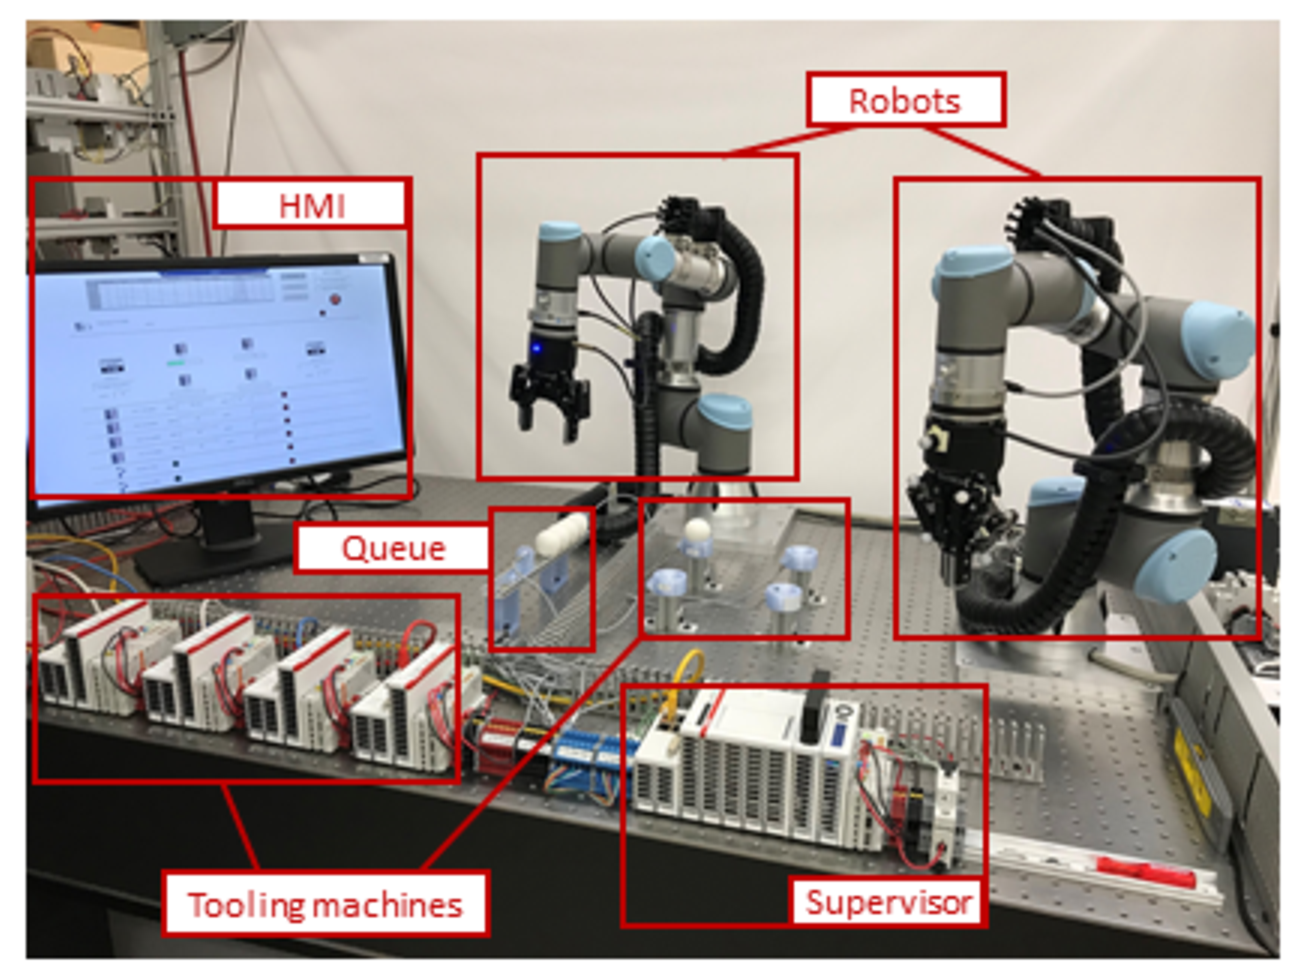
\includegraphics[width=\textwidth]{./chapter-gdb-appl/figures/cellShot}
	\caption{Collaborative work cell testbed}
	\label{gdbappl:fig::workcell}
\end{figure}

To facilitate wireless network research and showcase the power of wireless technologies in industrial practices, a testbed shown in Fig.~\ref{gdbappl:fig::workcell} has been developed at the National Institute of Standards and Technology (NIST) as described in~\cite{Liu2019vancouver}. The testbed is composed of two collaboration-grade robots, a supervisory programmable logic controller (PLC) used for the control of the workcell, four smaller PLCs serving as computer numerical control (CNC) machine emulators, and a human-machine interface (HMI).  Each robot is equipped with a six-degrees-of-freedom (DOF) force-torque (FT) sensor and a two-finger gripper. A Modbus/TCP server is included within the supervisor PLC and is used for communication between the supervisor and the robots.  The PLCs themselves communicate to each other using the Beckhoff Automation Device Specification (ADS) protocol. All elements within the workcell are synchronized to a stable and accurate grand-master clock. Therefore, as described in~\cite{Liu2019vancouver}, the operational, network, and measurement elements are all synchronized to the grand-master clock through a precision time protocol (PTP)-capable switch. 

Work-orders for the workcell are submitted through the supervisor. Each work-order consists of a work-plan for a part, and the work-plan determines how each part moves through the workcell until it is completed. The inspection of each part is conducted at each machining station, and after the final inspection, the part is placed back into the input queue.  Under normal operating conditions, the work continues until all work-orders have been processed.  This continuous form of operation provides ample opportunity to collect statistically significant metrics of both the network and the operation of the workcell.

\subsection{Database Schema}\label{gdbappl:sec::dbschema}

\begin{figure}[!ht]
	\centering
%	\includegraphics[width=\textwidth,trim=50 50 50 50, clip]{figures/database/arrows-schema.PNG}
	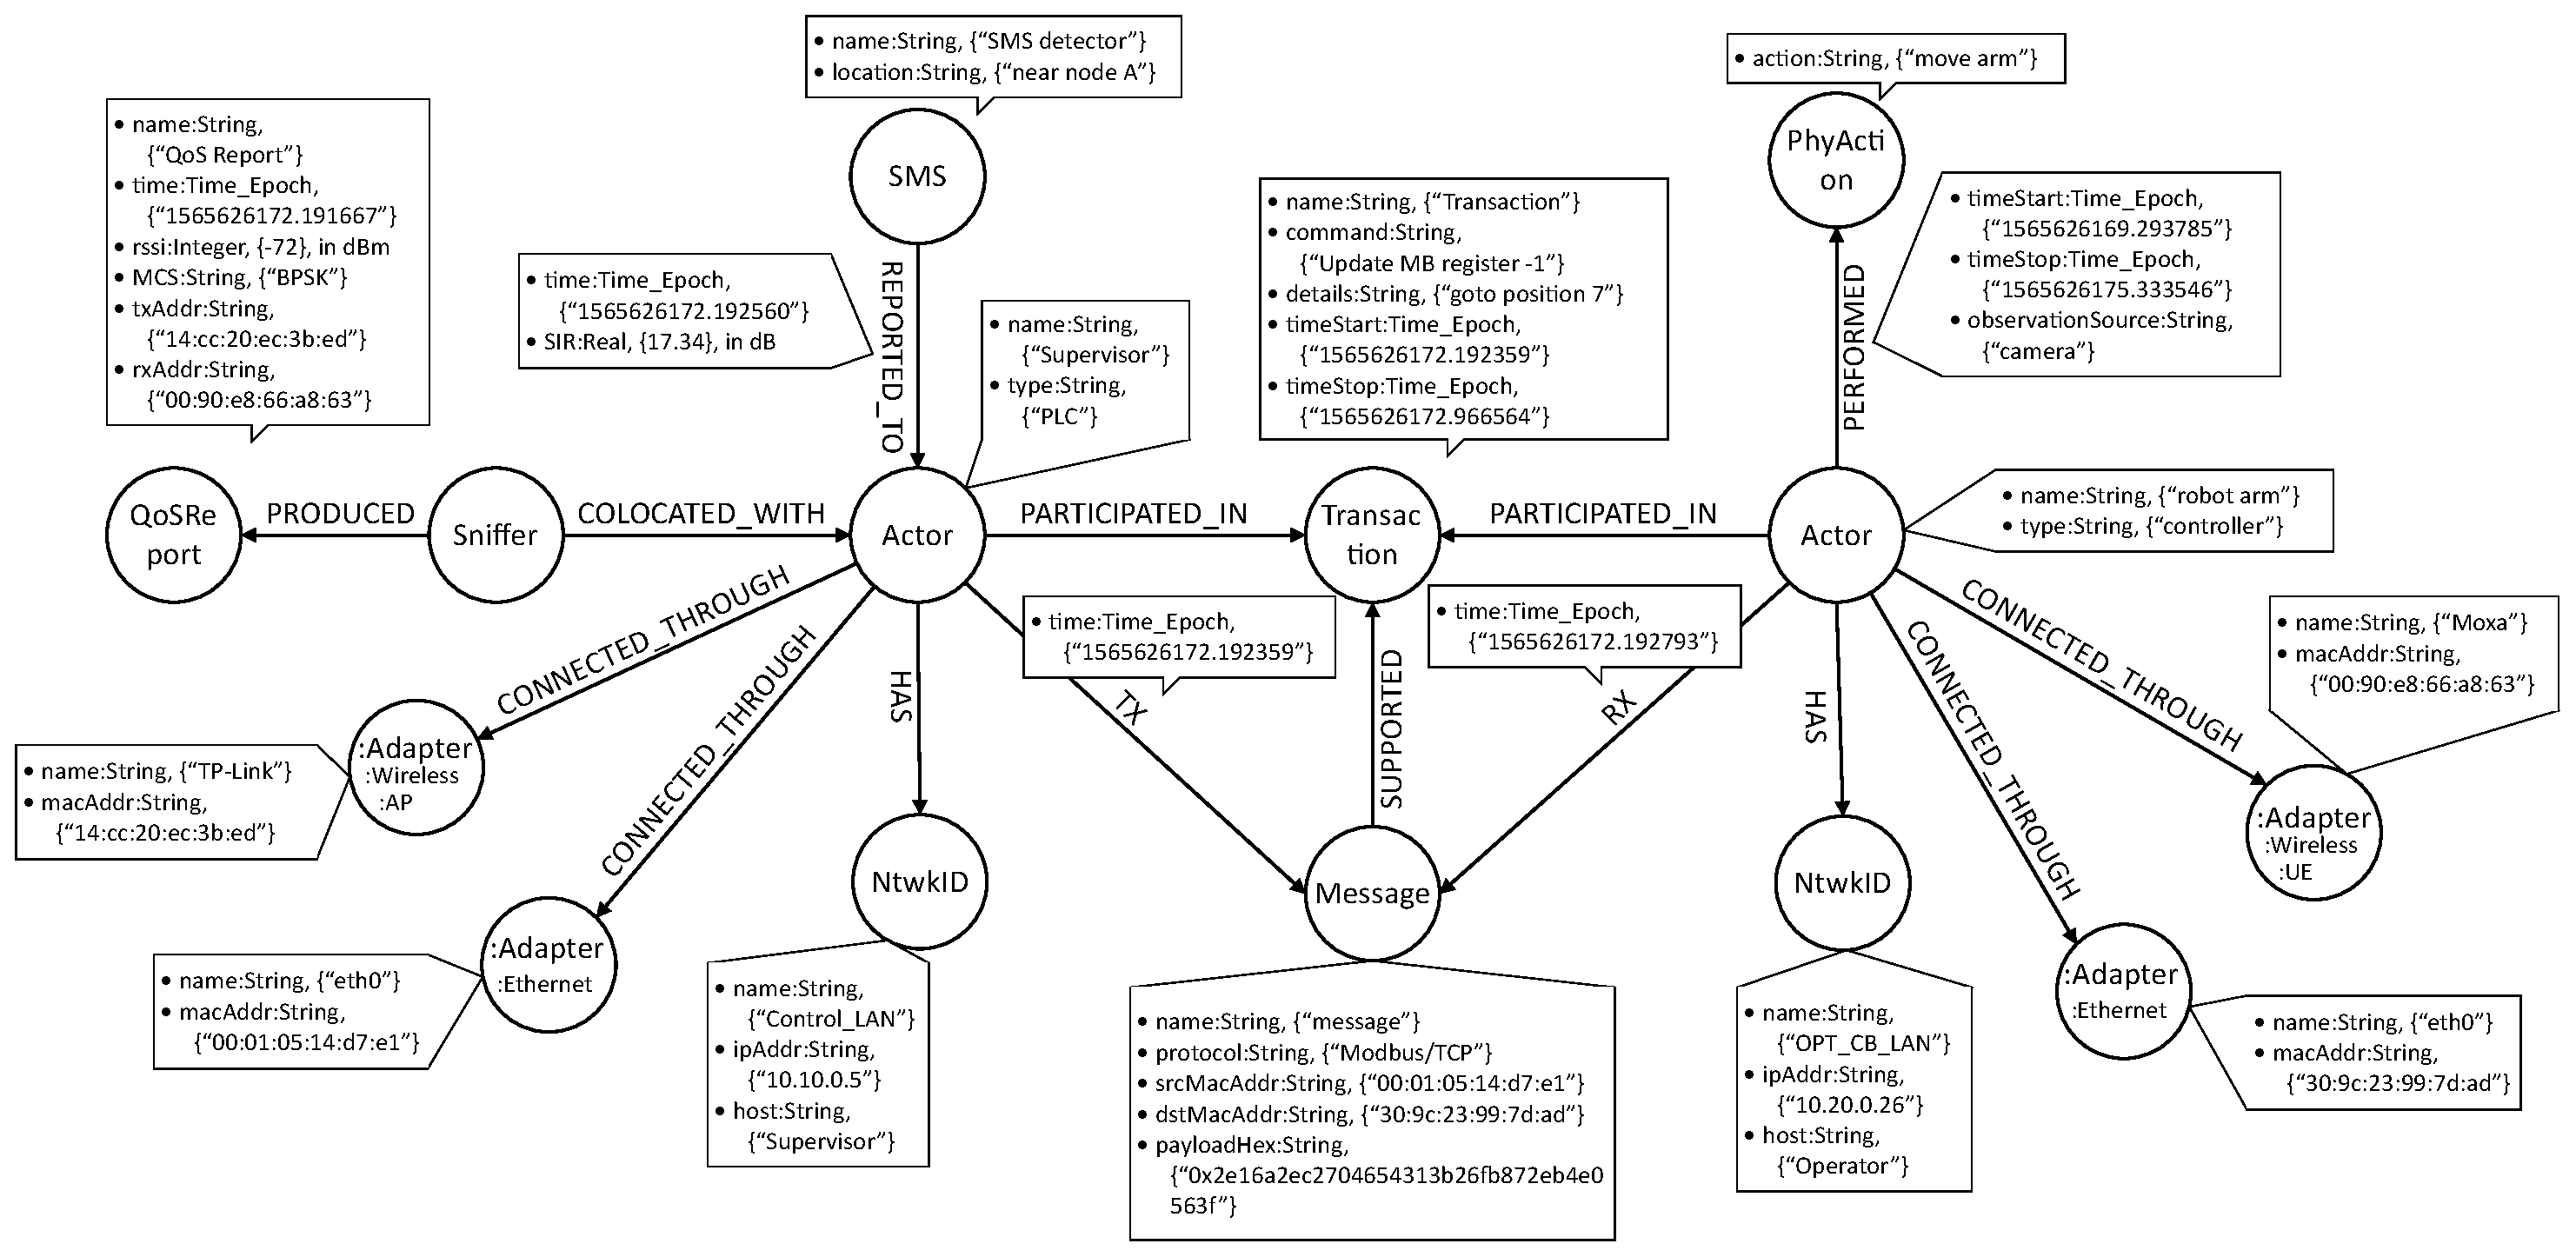
\includegraphics[width=\textwidth]{./chapter-gdb-appl/figures/database/graph_schema_0816.eps}
	\caption{The intended schema (i.e., pseudo-schema) of the graph database used for each operational run of the NIST wireless factory testbed.  The graph is organized into nodes and edges, where the edges signify relationships among network elements and physical operational elements.}
	\label{gdbappl:fig::database:schema}
\end{figure}

GDBs are NoSQL databases such that the database does not contain any predefined structure or rules to enforce such structure.  This is a major difference between relational databases and GDBs.  Nevertheless, it was necessary to sketch a pseudo-schema to capture the intended nodes and relationships that would be stored within the database (the terms pseudo-schema and schema will be used interchangeably). Before describing the schema itself, it is necessary to first explain the requirements of the schema.  Therefore, the requirements for our schema are as follows:

\begin{description}[style=sameline]
% [Time] 
\item[Time] Any manufacturing automation system is indeed a time-varying control system with network and operational events.  The database schema must necessarily support time-based queries and, specifically, time-windowed 
queries.
% [Operational Events]
\item[Operational Events] The schema must represent operational events such as the movement of a robot arm or the movement of a part.
% [Network Events]
\item[Network Events] The schema must represent network events such as the transmission of packets.
% [Transactions/Grouping]
\item[Message Grouping]  The schema must support grouping of logically related events such that those events can be correlated to a specific occurrence within the testbed.
% [Wired/Wireless Support]
\item[Wireless Support] The schema must support the capture of both wired and wireless network traffic without special provisions within queries for either.
% [QoS]
\item[QoS Support] The schema must allow for the capture of quality of service (QoS) data when available.
% [Spectrum Monitoring]
\item[Spectrum Monitoring] The schema must support the capture and association of network events with observations from a spectrum monitoring system (SMS) if that information is available.
\end{description}

\subsubsection{Node Design}

Given the fore-mentioned requirements, a sample pseudo-schema is shown in Fig.~\ref{gdbappl:fig::database:schema}, which represents the intended structure of the information within the GDB. It is important to remember that since GDB schemas are not really schemas, such as those found in relational databases, but representations of intent, the schema represented here should be considered a notional example of the final product.  Within the graphs, nodes represent logical elements, and edges represent the relationships between those elements.  Both nodes and edges may contain properties providing more description and labels that define categories or classes of the said nodes or edges.  Our schema is designed such that the data within the graph is intuitive to understand and allows for time-based queries to occur.  The facilitation of time-based queries was an essential requirement of our database design.  Our schema is represented using the following node labels:

\begin{description}[style=sameline]
    \item[Actor]  A physical component within the factory workcell such as a robot, PLC, or other networked item.
    \item[NtwkID] A network address item for an actor such as an Internet Protocol (IP) address.
    \item[Transaction] A complete information exchange between two or more actors (multiple actors may participate in a transaction).
    \item[Message] A network transmission event that occurs between two actors (messages are essentially packet transmissions captured at the transport layer; multiple messages support a transaction).
    \item[Physical Action]  A physical occurrence within a factory workcell associated with actors through multiple time based relationships.
    \item[SMS] An SMS observes and records significant spectral events within the workcell and may report those events to actors within the workcell.  
    \item[Sniffer] A measurement device that records all transmissions conducted over the wireless medium and includes wireless header information for each wireless transmission detected.
    \item[Adapter] A device that serves to connect an actor to a network (adapters are divided into sub-categories depending on the type of interface to a network).
    \item[Adapter:Ethernet] A subcategory of adapter representing an Ethernet interface. 
    \item[Adapter:Wireless] A subcategory of adapter representing a wireless interface. 
    \item[Adapter:Wireless:AP]  A subcategory of adapter representing a wireless access point interface.
    \item[Adapter:Wireless:UE] A subcategory of adapter representing a wireless user equipment interface.
    \item[QoS Report] A quality of service report of a message (not all messages will have a QoS report).
\end{description}

It is important to note that most network infrastructure components are not captured within the graph, but, instead, only basic interfaces between actors and the network are captured.  Our intent when designing the graph was to make the graph network and protocol agnostic, such that the network is viewed as a black-box. Accordingly, the captured events of the physical system and the network are considered useful for the analysis of performance. 

\subsubsection{Relationships (Graph Edges)}
Relationships are edges within the graph that capture the informational interactions between nodes.  Relationships, like nodes, can contain labels and properties.  As shown in Fig.~\ref{gdbappl:fig::database:schema}, nodes are connected through defined relationships.  A subset of the relationships are defined as follows:
\begin{description}
    \item[PARTICIPATED\_IN] Actors will participate in transactions.  A transaction exists for each logical set of messages between actors such as the setting of a Modbus register or the sending of a command to a robot.  Therefore, actors will participate in many transactions, and multiple actors may participate in a single transaction.
    \item[SUPPORTED] Messages (i.e., packets between actors) are associated with transactions through the SUPPORTED relationship. Depending on the protocol and the quality of the channel, a single transaction could have one or many messages connected through this relationship.
    \item[TX/RX] An actor may either transmit (TX) or receive (RX) a message. Both the TX and RX relationships contain a timestamp in the format of an epoch time which is a floating point number in seconds since January 1, 1970, with a resolution of microseconds.
    \item[PERFORMED] When an actor performs a physical action, a relationship is created between the actor and the physical action node. This relationship contains start and stop time properties as well as the source of the observation such as a networked camera.
    \item[REPORTED\_TO] An SMS may be a passive or active listener within a workcell.  When an SMS operates as an active listener, spectral reports from the SMS may be sent to an actor such that the actor can respond intelligently to the spectral event.  Reports from an SMS to an actor are captured within this relationship.
\end{description}
Other relationships shown in the schema of Fig.~\ref{gdbappl:fig::database:schema} but not explained above are considered self-explanatory.

\subsubsection{Closer Examination}
Examining the sample schema more closely, two actor nodes are represented.  In this case, Actor A is the supervisory controller, and Actor B is a robot arm.  Both nodes participate in a transaction, which, in this example, is a Modbus/TCP exchange. The transaction itself is associated with one or more messages (i.e., packets). Each message associated with a transaction manifests itself as a node in the graph. Multiple message nodes will exist for each transaction. 
%It is important to note that a timestamp is not recorded for each message.  The reason is that the timestamp for a message is captured in the edge relationships between the sender and the message and the receiver and the message.  Thus, a timestamp for transmission and reception are recorded within the graph through the TX/RX relationships.  
Additionally, QoS reports may be associated with each actor node through a collocated sniffer node.  By keeping QoS reports separate, we have the flexibility of supporting different wired and wireless protocols within the same graph. Recall, that a graph database has no enforceable structure and thus affords this type of flexibility. Each actor node may have network identities associated with it through the use of network identifier nodes.  Each network identifier node may contain address information such as a hardware address or a network address; however, this is dependent on the protocols and addressing schemes being used, and a node could have many different identification nodes. 
\subsubsection{Physical Actions}
Finally, each actor in the graph may associate with physical actions.  These actions exist in the database as automatons such that every time a new action occurs, a new edge would be added between the actor and the physical action.  Timestamps within the graph represent ``measurement time'' denoting that all  timestamps are accurately synchronized to the grand-master clock.  The method of synchronization is outside the scope of this paper and is explained fully in~\cite{Liu2019vancouver}.  This paper describes the database structure and the process for preparing and inserting the data into the database, which is described in the following subsection.

\subsection{Information Workflow}

\begin{figure*}[!ht]
    \centering
    \includegraphics[width=0.95\textwidth]{./chapter-gdb-appl/figures/database/work-flow.pdf}
    \caption{Data processing flow from factory workcell to database}
    \label{gdbappl:fig::work-flow}
\end{figure*}

The workflow for collecting, processing, and inserting measurement data into the graph database is multi-pronged, as shown in Fig.~\ref{gdbappl:fig::work-flow}.  The workcell, which in our case study is a two-robot workcell with four CNC machines, is instrumented with network probes that capture transmitted and received packets as well as probes to capture operational movements such as arm robot position and the state of the supervisor PLC.  Network data is stored in packet capture (PCAP) files, while operational data is stored in comma separated value (CSV) files. We developed bash scripts to extract relevant information and prepare the data for insertion into the database. The scripts also contain rules for grouping packets together as transactions based on the application protocol and time. The scripts produce CSV files that are ready for insertion into the Neo4j database.  Once the data resides within the database, we apply queries to extract information for the evaluation of workcell performance and visualization of network and operational events within the workcell. By tracking paths through the relationships within the graph, discerning how a network event such as interference is related to physical events such as position uncertainty or part throughput is possible. Various impairments may be introduced as a part of workcell operation.  Examples of such impairments include competing wireless traffic, radio interference, and reflections and diffraction due to the multi-path environment~\cite{Candell2017.NIST1951}. We have shown that it is feasible to implement such impairments and measure the resulting physical performance manifestation~\cite{Liu2019vancouver}. This is accomplished through the use of a radio channel emulator as demonstrated in~\cite{Candell2019vancouver}.

\subsection{Sample of a Resulting Graph}
In the following, we show results from a trial run of the NIST industrial wireless testbed. In this trial run, a single physical wireless link is used between a wireless adapter connected directly to the supervisor and a wireless access point connected to all the other actors in the testbed. The wireless nodes represent IEEE 802.11b/g/n devices and are connected through a variable radio frequency (RF) attenuator that allows us to vary the channel quality. During the trial run, the production of 10 parts was emulated, which resulted in 10 minutes of network activity.       

After populating the database with data captured from the trial run, the resulting realized schema is shown in Fig.~\ref{gdbappl:fig::real-schema}. The schema visualization is produced by invoking the command

\begin{lstlisting}
call db.schema.visualization()
\end{lstlisting} 
in Neo4j. It is important to note that a realized schema shows only one representation of each node and relationship whereas the intended pseudo-schema shown in Fig.~\ref{gdbappl:fig::database:schema} was developed to exemplify the relationships between types of nodes, labels, and relationships. Where label inheritance is employed, such as the case for different adapter types, relationships are reproduced; however, this is a result of the visualization tool rather than the schema itself.  Fig.~\ref{gdbappl:fig::real-schema} serves, therefore, to validate that the intended schema was indeed realized by the insertion of event data from the testbed. In the realized schema, inherited labels are shown as separate nodes.

\begin{figure}[!ht]
    \centering
    \includegraphics[width=0.99\columnwidth]{./chapter-gdb-appl/figures/database/graph_schema.png}
    \caption{Realized schema of the graph database fully populated after capturing network and operational data from the NIST industrial wireless testbed. }
    \label{gdbappl:fig::real-schema}
\end{figure}

As described in Section~\ref{gdbappl:sec::dbschema}, the database includes every network transaction that occurs during the operation of the testbed.  This includes any logical transaction nodes inserted into the database and any associated packets that happened to traverse the network.  Therefore, for a short duration of time depending on packet transmission rates, the amount of data stored in the database can grow quickly. This presents a visualization challenge that graphs are designed to handle. A sample graph is shown in Fig.~\ref{gdbappl:fig::Sample-graph_1}, which represents only 1 second of wired and wireless network data captured from the NIST two-robot pick-and-place wireless testbed described in~\cite{Liu2019vancouver}. 

\begin{figure}[!ht]
    \centering
   \includegraphics[width=0.95\textwidth]{./chapter-gdb-appl/figures/database/graph_M_T_2.png}
   \vspace{0.1in}
    \caption{ Visualization of a node graph resulting from a testbed experiment. }
    \label{gdbappl:fig::Sample-graph_1}
    \vspace{0.1in}
\end{figure}

This visualization is produced by calling the following query in the Neo4j. 
\begin{lstlisting}
MATCH p=(a:Actor {name:'Supervisor'})--(t:Transaction)--(b:Actor) ,p2=(m:Message)-->(t) WHERE t.timeStart>T AND t.timeStop<T+1
RETURN p,p2
\end{lstlisting}

The colors of the resulting nodes follow the realized schema in Fig.~\ref{gdbappl:fig::real-schema} while only the actors, transactions, and messages are visualized in Fig.~\ref{gdbappl:fig::Sample-graph_1}. The relationships between the messages and transactions are shown where a single transaction is connected to at least two messages to represent the communications between any two actors. The variable T in the query represents an arbitrary time variable in seconds within the trial run to capture the data within 1 second only.

We then show a more detailed visualization for all the nodes and relationships corresponding to a single transaction. This visualization is produced by calling the following query where Ts is an arbitrary time variable to specify the timeStart value for the single transaction. 

\begin{lstlisting}
MATCH p=(a:Actor {name:'Supervisor'})-->(t:Transaction {timeStart:Ts})<--(b:Actor {name:"CNC-1"})
WITH p, a, b, t
MATCH p1=(a)-->(m:Message)<--(b), p2=(m)-->(t), p3=(a)-[:HAS]-(),p4=(a)<-[:COLOCATED_WITH]-()-[:PRODUCED]->(q:QoSReport), p5=(a)-[:CONNECTED_THROUGH]-(),p6=(b)-[:HAS]-(), p7=(b)-[:CONNECTED_THROUGH]-()
WHERE q.time>t.timeStart AND q.time<t.timeStop
RETURN p,p1,p2,p3,p4,p5,p6,p7
\end{lstlisting}

In Fig.~\ref{gdbappl:fig::Sample-graph_2}, the actor nodes are labeled by their names \textit{CNC-1} and \textit{Supervisor}, the transaction is labeled by its type \textit{ADS}, the messages are labeled by their transmission role \textit{Request} and \textit{Response}, the NtwkIDs are labeled by their IP addresses, the Ethernet adapters are labeled by their names \textit{eth0}, the wireless adapters are labeled by their names \textit{Moxa} and \textit{TP-Link}, the sniffer is labeled by its name \textit{WLS1}, and the QoS reports are labeled by the received signal strength indicator (RSSI) value in dBm. This visualization includes only the QoS reports generated within the duration of the corresponding transaction.   

\begin{figure}[!ht]
    \centering
    \includegraphics[width=0.95\textwidth]{./chapter-gdb-appl/figures/database/graph_Single_trans.png}
    \caption{A detailed visualization resulting from a testbed experiment for all the nodes and relationships corresponding to a single transaction. }
    \label{gdbappl:fig::Sample-graph_2}
\end{figure}

\subsection{Calculation of Metrics}

\begin{figure}[!ht]
	\centering
%	\includegraphics[width=\textwidth,trim=50 50 50 50, clip]{figures/database/arrows-schema.PNG}
	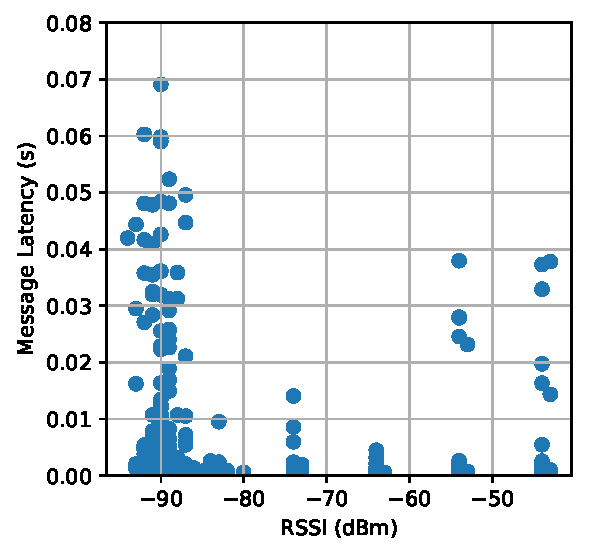
\includegraphics[width=0.5\textwidth]{./chapter-gdb-appl/figures/database/scatter_1.eps}
	\caption{Correlation between the message latency and the RSSI values by the sniffer.}
	\label{gdbappl:fig::database:scatter}
\end{figure}

We now present an example of deploying the proposed GDB approach in industrial wireless analysis. During the trial run time, we varied an RF attenuator value in the single wireless link. The attenuation can take the values \{0, 10, 20, 30, 40, 50, 60\} dB. We evaluate the message latency as the difference between the receive and transmit times of a message including transmission, processing, and retransmission times. Each message has been coupled to a QoS report that is the one reported at the closest time instant before the message transmit time. One of the parameters in the QoS report is the RSSI value captured by the Sniffer colocated with the supervisor's wireless adapter. 

In Fig.~\ref{gdbappl:fig::database:scatter}, we present a scatter plot showing the correlation between the message latency in seconds to the measured RSSI values by the sniffer in dBm.  The figure shows that the latency is higher at the lower RSSI values due to the increased number of retransmissions. Generally, an IEEE 802.11 transmission can occur using different IEEE 802.11 mode and modulation and coding scheme (MCS) based on the channel quality. At the RSSI of -90 dBm, the receiver should operate at the most robust communications mode and the lowest MCS index. However, retransmissions still occur due to having the received power near the sensitivity of the supervisor's wireless adapter. As shown in Fig.~\ref{gdbappl:fig::database:scatter}, retransmissions may occur at other RSSI values as well when the transmitter selects a higher mode of transmission and a higher MCS index. In this case, we assert that the receiver is operating close to the marginal sensitivity for a given mode (e.g., 802.11n) and MCS index.  We observed that the transmitter switches to a lower MCS index for the retransmitted messages, which supports our supposition. Therefore, latency can in fact be high for better RSSI values.  This effect is illustrated in Fig.~\ref{gdbappl:fig::database:scatter} where certain messages can have latency values at -43 dBm, which are comparable to those in the case of  -90 dBm.  

%SAMPLE CALCULATION FOR REDUCED GRAPH SHOWN ABOVE OVER A SMALL PERIOD OF TIME
%* network delay
%* correlate power level to delay
%* show the cypher command for computing this stuff

%TALK ABOUT LATER: SAMPLE CALCULATION OF PERFORMANCE DEPENDENCY OF THROUGHPUT TO NETWORK PERFORMANCE ON A SLIDING WINDOW

\section{Future Direction}

We have presented the general architecture of a performance evaluation database.  Future work will include developing query algorithms for the calculation of performance metrics as well as correlation of network events to the physical performance of the manufacturing system.  Algorithms will be developed to indicate locations in time of lost information making more direct performance correlations possible.  Beyond performance evaluation of the manufacturing system, we believe that the graph database approach enables anomaly detection because relationships within the data are intrinsically stored and thus efficiently queried.  The structure of the information is important within a graph database, and defining the relationships such that the paths through nodes may be discovered is essential to efficient queries and discovery of hidden correlations.  Therefore, more research will be done in the modification of the presented schema.  Machine learning will be applied for the detection of anomalies, performance degradation, signal quality, and network performance enhancement through more efficient resource allocation.  Our plans also include online database insertions to enable the demonstration of online operation of the database.   We also intend to examine the development of better control system strategies that mitigate network losses and delays.  Since this approach is indifferent to the communications  protocols used, we intend to extend our database approach to include various protocols, radio bands such as millimeter wave bands for 5G communications, and different use cases to include mobile robotic platforms and safety critical systems.

\section{Conclusions} \label{gdbappl:sec::conclusion}
We have presented in this paper a novel approach to capturing network and operational event information from a factory workcell with the  purposes of 1) capturing and storing of network and operational events, 2) calculating performance metrics of the network, and 3) discovering performance dependencies between the network and the physical assembly of the workcell.  Using a graph database, we have demonstrated that it is possible to construct such a database, compute network performance metrics and discover correlations.  We have also developed the capability of examining the correlation between network events and the performance of physical actions.  This will be a source of further research.

Future progress and measurement data will be deposited in the NIST public domain repository as a reference for industrial traffic modeling efforts and comparative studies on industrial wireless technologies~\cite{Candell2019PROJECTURL}.



% references section
%\bibliography{chapter-gdb-appl/gdb-appl}




\chapter{Conclusions}

paper on testbed construction; ground truth; data sources network and physical; data outputs; 

paper on graph database approach for organization of data

Discussion, Perspectives, restate findings


% Automatic Lettrine and Minitoc at the begining of the chapter.
%
% The following macros are formatting the text at the begining of a chapter according to the
% standard format.
%
% \chapterintro               See \chapterintrotosection.
%
% \chapterintro*              Similar to \chapterintro, except that the minitoc will be ignored.
%
% \chapterintrotosection      transform to lettrine the first letter that is following this macro
%                             until the next following \section macro.
%                             YOU MUST type the \section macro
%                             in the same file as the \chapterintrotosection macro.
%                             AND
%                             put a minitoc (if the minitoc package is included) just before
%                             the next following \section macro.
%
% \chapterintrotoinput        transform to lettrine the first letter that is following this macro
%                             until the next following \input macro.
%                             YOU MUST type the \input macro
%                             in the same file as the \chapterintrotoinput macro.
%                             AND
%                             put a minitoc (if the minitoc package is included) just before
%                             the next following \input macro.
%
% \chapterintrotoinclude      transform to lettrine the first letter that is following this macro
%                             until the next following \include macro.
%                             YOU MUST type the \include macro
%                             in the same file as the \chapterintrotoinclude macro.
%                             AND
%                             put a minitoc (if the minitoc package is included) just before
%                             the next following \include macro.

%\chapterintro*
%\chapterintro
%\chapterintrotosection
%\chapterintrotoinput
%\chapterintrotoinclude




 
%%--------------------
%% Start the end of the thesis
\iftoggle{usingspim}{
\backmatter
}
 
%%--------------------
%% Bibliography
 
%% PERSONAL BIBLIOGRAPHY (use 'multibib')
 
%% Change the style of the PERSONAL bibliography
%\bibliographystylePERSO{phdthesisapa}
 
%% Add the chapter with the PERSONAL bibliogaphy.
%% The name of the BibTeX file may be the same as
%% the one for the general bibliography.
%\bibliographyPERSO{biblio.bib}
 
%% Below, include a chapter for the GENERAL bibliography.
%% It is assumed that the standard BibTeX tool/approach
%% is used.
 
%% GENERAL BIBLIOGRAPHY
 
%% To cite one of your PERSONAL papers with the style
%% of the PERSONAL bibliography: \cite{key}
 
%% To force to show one of your PERSONAL papers into
%% the PERSONAL bibliography, even if not cited in the
%% text: \nocite{key}
 
%% The following line set the style of
%% the GENERAL bibliogaphy.
%% The "phdthesisapa" is a "apalike" style with the following
%% differences:
%% a) The titles are output with the color of the institution.
%% b) The name of the PhD thesis' author is underlined.
%\bibliographystyle{phdthesisnum}
%% The following line may be used in place of the previous
%% line if you prefer "numeric" citations.
\bibliographystyle{phdthesisnum}
 
%% Link the GENERAL bibliogaphy to a BibTeX file.
%\bibliography{biblio.bib}
%\bibliographystyle{IEEEtran.bib}
 
%%--------------------
%% List of figures and tables

\iftoggle{usingspim}{
 
%% Include a chapter with a list of all the figures.
%% In French typograhic standard, this list must be at
%% the end of the document.
\listoffigures
 
%% Include a chapter with a list of all the tables.
%% In French typograhic standard, this list must be at
%% the end of the document.
\listoftables
 
%%--------------------
%% Include a list of definitions
\listofdefinitions

}

%%--------------------
%% Appendixes
\appendix
\part{Annexes}
 
\chapter{Premier chapitre des annexes}

\chapter{Second chapitre des annexes}
 
\end{document}
